\documentclass[12pt,a4paper]{article}
\usepackage[a4paper, margin=0.8in, headheight=14pt]{geometry}
\usepackage{fontspec}
\usepackage{unicode-math}
\setmainfont{TeX Gyre Pagella}
\setmonofont[Scale=0.88]{TeX Gyre Cursor}
\setmathfont{Latin Modern Math}
\usepackage{xcolor}
\usepackage{colortbl}
\usepackage{titlesec}
\usepackage{enumitem}
\usepackage{tabularx}
\usepackage{booktabs}
\usepackage{array}
\usepackage{amsmath}
\allowdisplaybreaks
\usepackage{tikz}
\usetikzlibrary{shapes.geometric, arrows.meta, positioning, calc, fit, decorations.pathreplacing, decorations.pathmorphing, patterns, backgrounds}
% circuitikz not required for this subject
\usepackage{tcolorbox}
\tcbuselibrary{skins, breakable}
\usepackage{etoolbox}
\usepackage{hyperref}
\usepackage{fancyhdr}
\usepackage{graphicx}
\usepackage{microtype}
\hyphenpenalty=10000
\exhyphenpenalty=10000
\sloppy
\usepackage{caption}
\usepackage{setspace}
\usepackage{multirow}
\usepackage{tocloft}
\newcommand{\Q}[1]{\textbf{#1}\par\noindent\ignorespaces}
\definecolor{myred}{RGB}{196,30,58}
\definecolor{mydark}{RGB}{30,30,50}
\definecolor{mygreen}{RGB}{14,120,80}
\definecolor{myteal}{RGB}{0,130,140}
\definecolor{myamber}{RGB}{180,100,0}
\definecolor{mypurple}{RGB}{100,30,160}
\definecolor{mygray}{RGB}{246,247,249}
\definecolor{mgframe}{RGB}{180,185,200}
\definecolor{watermark}{RGB}{145,150,170}
\definecolor{hdrred}{RGB}{250,232,235}
\definecolor{hdrgreen}{RGB}{220,244,233}
\definecolor{hdrteal}{RGB}{220,242,244}
\definecolor{hdramber}{RGB}{253,242,215}
\definecolor{hdrpurple}{RGB}{238,228,255}
\definecolor{hdrgray}{RGB}{238,240,245}
\definecolor{rowalt}{RGB}{250,251,253}
\AfterEndEnvironment{tcolorbox}{\color{mydark}}

\titleformat{\section}{\large\bfseries\color{myred}}{\thesection.}{0.5em}{}[\vspace{1pt}{\color{myred}\rule{\linewidth}{0.8pt}}]
\titleformat{\subsection}{\normalsize\bfseries\color{myteal}}{\thesubsection}{0.5em}{}
\titlespacing*{\section}{0pt}{18pt}{7pt}
\titlespacing*{\subsection}{0pt}{11pt}{4pt}
\setlength{\parindent}{0pt}
\setlength{\parskip}{4pt}
\renewcommand{\cfttoctitlefont}{\large\bfseries\color{myred}}
\renewcommand{\cftaftertoctitle}{\par\noindent{\color{myred}\rule{\linewidth}{0.8pt}}}
\setlength{\cftbeforetoctitleskip}{0pt}
\setlength{\cftaftertoctitleskip}{6pt}
\renewcommand{\cftsecfont}{\normalsize\bfseries\color{mydark}}
\renewcommand{\cftsecpagefont}{\normalsize\bfseries\color{mydark}}
\renewcommand{\cftsecleader}{\cftdotfill{\cftdotsep}}
\setlength{\cftbeforesecskip}{7pt}
\renewcommand{\cftsubsecfont}{\small\color{mydark}}
\renewcommand{\cftsubsecpagefont}{\small\color{mydark}}
\setlength{\cftbeforesubsecskip}{3pt}
\setlength{\cftsubsecindent}{1.4em}
\renewcommand{\cftpartfont}{\normalsize\bfseries\color{myteal}}
\renewcommand{\cftpartpagefont}{\normalsize\bfseries\color{myteal}}
\setlength{\cftbeforepartskip}{14pt}
\renewcommand{\arraystretch}{1.45}
\setlength{\tabcolsep}{6pt}
\arrayrulecolor{mydark}
\newcolumntype{B}[1]{>{\small\bfseries\raggedright\arraybackslash}m{#1}}
\newcolumntype{C}[1]{>{\centering\arraybackslash}m{#1}}
\newcolumntype{Y}{>{\small\raggedright\arraybackslash}X}
\renewcommand{\tabularxcolumn}[1]{m{#1}}
\newcommand{\currmodule}{Module 1}
\pagestyle{fancy}
\fancyhf{}
\fancyhead[L]{\small\color{myred}\textbf{EC401}\;\color{mydark}--- Analog Communication}
\fancyhead[R]{\small\color{myteal}\textbf{\currmodule\ Notes}}
\fancyfoot[C]{\small\color{mydark}\thepage}
\fancyfoot[R]{\small\color{watermark}\textit{\copyright\ Biraj}}
\renewcommand{\headrulewidth}{0.5pt}
\renewcommand{\footrulewidth}{0.3pt}

\hypersetup{colorlinks=true, linkcolor=myteal, urlcolor=myteal,
  pdfauthor={Biraj Sarkar},
  pdftitle={EC401 --- Combined Notes}}

\tcbset{
  tikzbox/.style={
    colback=mygray, colframe=mgframe, boxrule=0.6pt, arc=4pt,
    left=8pt, right=8pt, top=6pt, bottom=6pt,
    colbacktitle=mgframe, coltitle=mydark, fonttitle=\small\bfseries
  },
  defbox/.style={
    colback=hdrgreen, colframe=mygreen, boxrule=0.8pt, arc=4pt,
    left=9pt, right=9pt, top=6pt, bottom=6pt,
    colbacktitle=mygreen, coltitle=white, fonttitle=\small\bfseries
  },
  formulabox/.style={
    colback=hdrteal, colframe=myteal, boxrule=0.8pt, arc=4pt,
    left=9pt, right=9pt, top=7pt, bottom=7pt,
    colbacktitle=myteal, coltitle=white, fonttitle=\small\bfseries
  },
  examplebox/.style={
    colback=hdramber, colframe=myamber, boxrule=0.8pt, arc=4pt,
    left=9pt, right=9pt, top=6pt, bottom=6pt,
    colbacktitle=myamber, coltitle=white, fonttitle=\small\bfseries
  },
  masonbox/.style={
    colback=hdrpurple, colframe=mypurple, boxrule=0.8pt, arc=4pt,
    left=9pt, right=9pt, top=6pt, bottom=6pt,
    colbacktitle=mypurple, coltitle=white, fonttitle=\small\bfseries
  },
  exambox/.style={
    colback=hdrpurple, colframe=mypurple, boxrule=1pt, arc=5pt,
    left=10pt, right=10pt, top=8pt, bottom=8pt,
    colbacktitle=mypurple, coltitle=white, fonttitle=\bfseries,
    breakable, title after break={\textbf{Frequently Asked / Viva Questions (contd.)}}
  }
}
\tcbset{breakable}
\tcbset{coltext=mydark}
\tcbset{after={\color{mydark}}}

\tikzset{
  block/.style={rectangle, draw=myteal, fill=hdrteal,
    text width=2.4cm, align=center, minimum height=0.95cm,
    font=\small, rounded corners=3pt, line width=0.7pt},
  redblock/.style={rectangle, draw=myred, fill=hdrred,
    text width=2.4cm, align=center, minimum height=0.95cm,
    font=\small, rounded corners=3pt, line width=0.7pt},
  netnode/.style={rectangle, draw=myteal, fill=hdrteal,
    text width=1.5cm, align=center, minimum height=0.8cm,
    font=\small, rounded corners=3pt, line width=0.7pt},
  sumjunc/.style={circle, draw=myamber, fill=hdramber,
    minimum size=0.62cm, font=\small, line width=0.8pt},
  snode/.style={circle, draw=mypurple, fill=hdrpurple,
    minimum size=0.55cm, font=\footnotesize, line width=0.7pt},
  arrow/.style={-Stealth, thick, color=mydark},
  redarrow/.style={-Stealth, thick, color=myred},
  line/.style={thick, color=mydark}
  % ⚠ Do NOT define axis/.style here — conflicts with pgfplots/library keys.
  %   Use inline style instead: \draw[-Stealth, thin, color=mydark]
}

\newcommand{\modulestart}[2]{%
  \clearpage
  \renewcommand{\currmodule}{Module #1}%
  \renewcommand{\theHsection}{mod#1.\arabic{section}}%
  \renewcommand{\theHsubsection}{\theHsection.\arabic{subsection}}%
  \renewcommand{\theHsubsubsection}{\theHsubsection.\arabic{subsubsection}}%
  \phantomsection
  \addcontentsline{toc}{part}{Module #1: #2}%
  \setcounter{section}{0}%
  \begin{center}
    \vspace*{1.0cm}
    {\Huge\bfseries\color{myred} Module #1}\\[10pt]
    {\Large\bfseries\color{mydark} #2}\\[10pt]
    {\color{myred}\rule{0.55\linewidth}{1.2pt}}
  \end{center}
  \vspace{14pt}
}
\begin{document}

\thispagestyle{empty}

% ─── Page Border (TikZ Overlay) ────────────────────────────────────────────────
\begin{tikzpicture}[remember picture, overlay]
  % Outer border (fine line in mgframe)
  \draw[color=mgframe, line width=1.5pt] 
    ($(current page.north west) + (0.6in, -0.6in)$) rectangle 
    ($(current page.south east) + (-0.6in, 0.6in)$);
  % Inner border (finer accent line in myred)
  \draw[color=myred, line width=0.8pt] 
    ($(current page.north west) + (0.65in, -0.65in)$) rectangle 
    ($(current page.south east) + (-0.65in, 0.65in)$);
\end{tikzpicture}

\vspace*{1.0cm}
\begin{center}
  {\Huge\bfseries\color{myred} EC401}\\[10pt]
  {\LARGE\bfseries\color{mydark} Analog Communication}\\[20pt]
  {\color{myred}\rule{0.7\linewidth}{1.5pt}}\\[18pt]
  {\Large\color{myteal}\textbf{Combined Module Notes}}\\[8pt]
  {\large\color{mydark} Modules 1 -- 4}\\[40pt]
  {\normalsize\color{mydark} Semester IV \quad$\bullet$\quad ECE \quad$\bullet$\quad 3 Credits}\\[12pt]
  {\normalsize\color{mydark} CGEC \;$|$\; B.Tech ECE (2023--27)}
\end{center}
\vspace{1.0cm}
\begin{center}
  \begin{tcolorbox}[colback=mygray, colframe=mgframe, boxrule=0.5pt, arc=3pt, width=0.85\linewidth]
    \centering\small\color{mydark}
    \textbf{Disclaimer / Study Guide Notice:}\\
    These are condensed \textbf{Short Notes} focusing on core theory, key formulas, block/circuit diagrams, and standard viva Q\&As for university exam revision. Exhaustive numerical practice problems and derivation edge cases are not covered. This serves as a quick-revision reference guide for students.
  \end{tcolorbox}
\end{center}
\vfill
\vspace{0.6cm}
\begin{center}
  {\large\bfseries\color{mypurple} Biraj Sarkar}\\[16pt]
  {\footnotesize\color{watermark}\textbf{IN ASSOCIATION WITH}}\\[8pt]
  {\small\bfseries\color{mydark} MAKAUT Wingman \quad$\bullet$\quad MAKAUT Future Minds}\\[12pt]
  {\large\bfseries\color{myteal} Cooch Behar Government Engineering College}
\end{center}
\vfill
\begin{center}{\small\color{watermark}\textit{Exam-Ready Notes}}\end{center}
\clearpage

\hypersetup{linkcolor=mydark}
\tableofcontents
\hypersetup{linkcolor=myteal}
\clearpage

% -- Module 1 -----------------------------------------------------------------
\modulestart{1}{Introduction to Analog Communication}

\section{Introduction to Analog Communication}

\begin{tcolorbox}[defbox, title={Communication System and Modulation}]
An analog communication system carries a continuously varying message from source to destination. The transmitter converts the message to a suitable electrical waveform, modulates a carrier and provides power for transmission. The channel (free space, cable or another medium) introduces attenuation, distortion and noise. The receiver selects and amplifies the desired signal, demodulates it and drives the output transducer.
\end{tcolorbox}

\begin{tcolorbox}[tikzbox, unbreakable, title={Transmitter, Channel and Receiver}]
\centering
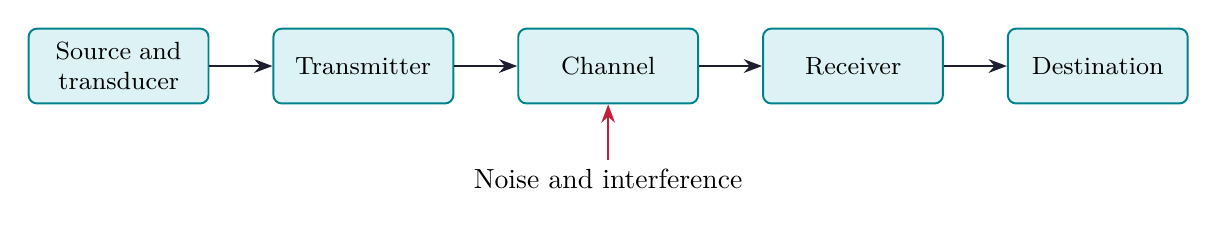
\begin{tikzpicture}[node distance=8mm,sblock/.style={block,text width=2.05cm}]
  \node[sblock] (src) {Source and transducer};
  \node[sblock,right=of src] (tx) {Transmitter};
  \node[sblock,right=of tx] (ch) {Channel};
  \node[sblock,right=of ch] (rx) {Receiver};
  \node[sblock,right=of rx] (dst) {Destination};
  \draw[arrow] (src)--(tx);
  \draw[arrow] (tx)--(ch);
  \draw[arrow] (ch)--(rx);
  \draw[arrow] (rx)--(dst);
  \node[below=7mm of ch] (noise) {Noise and interference};
  \draw[redarrow] (noise)--(ch);
\end{tikzpicture}\par
\end{tcolorbox}

\subsection{Concept of Modulation and Need for Modulation}
Modulation is the systematic variation of one or more parameters (amplitude, phase, or frequency) of a high-frequency carrier signal in accordance with the instantaneous value of a baseband message signal $m(t)$. Baseband signals cannot be transmitted directly through free space. Five critical engineering reasons mandate modulation:

\begin{enumerate}[leftmargin=1.5em, itemsep=3pt]
  \item \textbf{Practicable Antenna Dimensions}: For efficient radiation, an antenna length must be of the order of a quarter wavelength ($\ell \ge \lambda/4 = c/(4f)$). Directly transmitting a baseband audio tone of $5\,\mathrm{kHz}$ requires $\ell = 3\times10^8/(4\times5\times10^3) = 15\,\mathrm{km}$, which is physically unrealizable. Translating to an RF carrier of $1\,\mathrm{MHz}$ reduces the required length to $\ell = 75\,\mathrm{m}$, which is readily constructed.
  \item \textbf{Multiplexing (Frequency Division Multiplexing)}: Baseband audio signals from all sources occupy the identical spectral range ($20\,\mathrm{Hz}$--$20\,\mathrm{kHz}$). Direct transmission over a common wireless medium causes complete mutual interference and unintelligible reception. Modulation translates each message to a distinct non-overlapping frequency slot ($f_{c1}, f_{c2}, \dots$), permitting simultaneous multichannel broadcast.
  \item \textbf{Narrowbanding and Fractional Bandwidth}: An antenna cannot maintain impedance matching across a wide frequency ratio. Baseband audio spans $20\,\mathrm{Hz}$ to $20\,\mathrm{kHz}$ (a $1000:1$ ratio). When modulated onto a $1\,\mathrm{MHz}$ carrier, the occupied passband is $0.98$--$1.02\,\mathrm{MHz}$, yielding a fractional bandwidth of only $20\,\mathrm{kHz}/1\,\mathrm{MHz} = 2\%$, easily tuned by a single resonant circuit.
  \item \textbf{Antenna Radiation Efficiency}: Radiated power from an antenna of physical length $\ell$ obeys $P_{\mathrm{rad}} \propto (\ell/\lambda)^2$. At low baseband frequencies, $\lambda$ is tens of kilometers, making $(\ell/\lambda)^2 \to 0$ and converting almost all power into thermal losses. Raising the carrier frequency makes $\lambda$ small, maximizing radiated power.
  \item \textbf{Noise and Interference Immunity}: Audio frequencies suffer heavily from industrial $50\,\mathrm{Hz}$ power hum, atmospheric noise, and semiconductor $1/f$ flicker noise. Translating to RF moves the transmission into low-noise spectral windows.
\end{enumerate}

\begin{tcolorbox}[examplebox, title={Quarter-Wave Antenna Dimension Calculation}]
Compare the physical quarter-wave vertical antenna lengths required for direct audio transmission versus RF carrier transmission ($c=3\times10^8\,\mathrm{m/s}$):
\[
\begin{aligned}
 \ell&=\frac{\lambda}{4}=\frac{c}{4f},\\
 \text{Audio tone ($f_m = 5\,\mathrm{kHz}$):}\quad \ell_{\mathrm{audio}}&=\frac{3\times10^8}{4(5\times10^3)}\,\mathrm{m} = 15\,000\,\mathrm{m} = 15\,\mathrm{km},\\
 \text{RF carrier ($f_c = 1\,\mathrm{MHz}$):}\quad \ell_{\mathrm{RF}}&=\frac{3\times10^8}{4(10^6)}\,\mathrm{m} = 75\,\mathrm{m},\\
 \text{VHF FM ($f_c = 100\,\mathrm{MHz}$):}\quad \ell_{\mathrm{VHF}}&=\frac{3\times10^8}{4(10^8)}\,\mathrm{m} = 0.75\,\mathrm{m} = 75\,\mathrm{cm}.
\end{aligned}
\]
Modulation reduces antenna height from an impossible $15\,\mathrm{km}$ tower to a convenient $75\,\mathrm{cm}$ rod.
\end{tcolorbox}

\subsection{Baseband, Passband and Channel Selection}
A microphone or sensor produces a \textbf{baseband} waveform whose useful frequencies extend from near DC to $W$. The transmitter translates the message around an allocated RF carrier $f_c$. A channel of usable bandwidth $B_{\rm ch}$ must pass the resulting spectrum. An RF filter at the receiver selects the channel before demodulation, and a baseband low-pass filter extracts the recovered message.

\begin{tcolorbox}[formulabox, title={Why Carrier Multiplication Shifts the Spectrum}]
For $\mathcal F\{m(t)\}=M(f)$ and angular frequency $\omega_c=2\pi f_c$,
\[
\begin{aligned}
 m(t)\cos\omega_ct
   &=\tfrac12m(t)e^{j\omega_ct}+\tfrac12m(t)e^{-j\omega_ct},\\
 \mathcal F\{m(t)\cos\omega_ct\}
   &=\tfrac12M(f-f_c)+\tfrac12M(f+f_c).
\end{aligned}
\]
The positive-frequency copy lies between $f_c-W$ and $f_c+W$. For example, a message limited to $4\,\mathrm{kHz}$ sent on a $200\,\mathrm{kHz}$ carrier occupies $196$--$204\,\mathrm{kHz}$ before any guard bands are added. Its negative-frequency mirror is required because the time waveform is real.
\end{tcolorbox}

A nearly flat gain and approximately linear phase over the occupied band preserve the waveform shape up to gain and delay. A selective notch inside a sideband removes particular message components. This is why frequency allocation, channel selectivity and modulation bandwidth have to be considered together.

\section{Conventional AM with Transmitted Carrier}
The transmitter sends a carrier alongside two shifted versions of the message. This allows a simple receiver to recover the audio from the envelope.

\subsection{Time-Domain Expression and Envelope}

\begin{tcolorbox}[defbox, title={Double Sideband with Transmitted Carrier (DSB-TC)}]
For carrier peak $A_c$ in volts, carrier frequency $f_c$ in hertz and sensitivity $k_a$ in $\mathrm{V^{-1}}$,
\[
s(t)=A_c[1+k_a m(t)]\cos(2\pi f_ct).
\]
For a tone $m(t)=A_m\cos(2\pi f_mt)$, $\mu=k_aA_m$ is the dimensionless modulation index. The signed envelope factor is $1+\mu\cos(2\pi f_mt)$.
\end{tcolorbox}

Using $\cos a\cos b=\tfrac12[\cos(a+b)+\cos(a-b)]$,
\[
\begin{aligned}
 s(t)&=A_c\cos(2\pi f_ct)+\mu A_c\cos(2\pi f_mt)\cos(2\pi f_ct)\\
     &=A_c\cos(2\pi f_ct)\\
     &\quad+\frac{\mu A_c}{2}\cos[2\pi(f_c+f_m)t]\\
     &\quad+\frac{\mu A_c}{2}\cos[2\pi(f_c-f_m)t].
\end{aligned}
\]
The upper and lower sidebands (USB and LSB) are at $f_c+f_m$ and $f_c-f_m$. Each has peak voltage $\mu A_c/2$.

\subsection{Spectrum and Bandwidth}
With the transform kernel $e^{-j2\pi ft}$, a cosine of peak $A$ contributes two impulses of weight $A/2$. With $M(f)$ supported on $|f|\le W$,
\[
\begin{aligned}
 S(f)&=\frac{A_c}{2}[\delta(f-f_c)+\delta(f+f_c)]\\
     &\quad+\frac{k_a A_c}{2}[M(f-f_c)+M(f+f_c)],\\
 B_{\mathrm{AM}}&=(f_c+W)-(f_c-W)=2W\quad(\mathrm{Hz}).
\end{aligned}
\]
For a tone the carrier impulses have weight $A_c/2$ each, and the four sideband impulses have weight $\mu A_c/4$ each.

\begin{tcolorbox}[tikzbox, unbreakable, title={Two-Sided Spectrum of Single-Tone AM}]
\centering
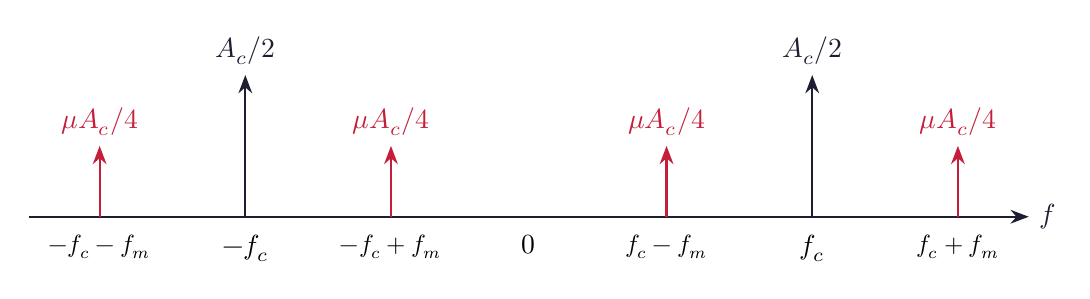
\begin{tikzpicture}
 \draw[arrow] (-6.35,0)--(6.35,0) node[right] {$f$};
 \node[below=3pt] at (0,0) {$0$};
 \foreach \x/\ff in {-3.6/-f_c,3.6/f_c}{
   \draw[arrow] (\x,0)--(\x,1.8) node[above] {$A_c/2$};
   \node[below=3pt] at (\x,0) {$\ff$};
 }
 \foreach \x/\ff in {-5.45/-f_c-f_m,-1.75/-f_c+f_m,1.75/f_c-f_m,5.45/f_c+f_m}{
   \draw[redarrow] (\x,0)--(\x,0.9) node[above] {$\mu A_c/4$};
   \node[below=3pt] at (\x,0) {\small $\ff$};
 }
\end{tikzpicture}\par
\end{tcolorbox}

\subsection{Carrier-Referenced Phasors}
In a frame rotating at $2\pi f_c$, the carrier is stationary. The USB and LSB rotate in opposite directions at $2\pi f_m$. Their transverse components cancel. Their horizontal components add to $\mu A_c\cos(2\pi f_mt)$.

\begin{tcolorbox}[tikzbox, unbreakable, title={AM Phasors at a Representative Instant}]
\centering
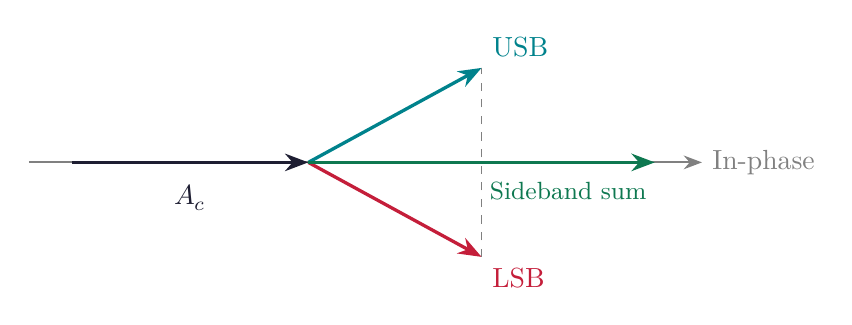
\begin{tikzpicture}
 \draw[arrow,gray] (-0.55,0)--(8.0,0) node[right] {In-phase};
 \draw[arrow,very thick] (0,0)--(3,0) node[midway,below=4pt] {$A_c$};
 \draw[arrow,myteal,very thick] (3,0)--(5.2,1.2) node[above right] {USB};
 \draw[redarrow,very thick] (3,0)--(5.2,-1.2) node[below right] {LSB};
 \draw[dashed,gray] (5.2,-1.2)--(5.2,1.2);
 \draw[arrow,mygreen,very thick] (3,0)--(7.4,0);
 \node[mygreen,below] at (6.3,-0.12) {\small Sideband sum};
\end{tikzpicture}\par
\small Both sideband vectors have magnitude $\mu A_c/2$. Their projections add to the in-phase carrier.
\end{tcolorbox}

\subsection{Under-, Critical and Overmodulation}
The magnitude envelope is $A_c|1+\mu\cos(2\pi f_mt)|$. For $\mu<1$ it stays positive. At $\mu=1$ it touches zero. For $\mu>1$ the signed factor becomes negative near the trough, reversing RF phase by $\pi$. Envelope detection folds this interval, causing distortion.

\begin{tcolorbox}[tikzbox, unbreakable, title={Signed Envelope Factor at Three Modulation Depths}]
\centering
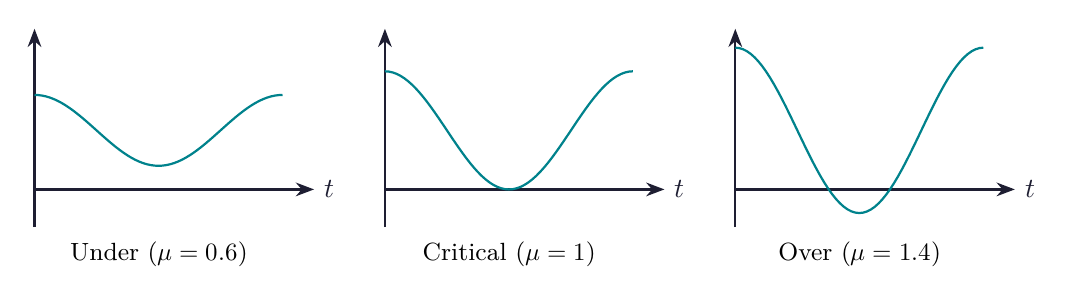
\begin{tikzpicture}
 \foreach \offset/\depth/\label in {0/0.6/Under,4.45/1/Critical,8.9/1.4/Over}{
   \begin{scope}[shift={(\offset,0)}]
    \draw[arrow] (0,0)--(3.55,0) node[right] {$t$};
    \draw[arrow] (0,-0.48)--(0,2.04);
    \draw[myteal,thick,domain=0:3.15,samples=65]
      plot (\x,{0.75*(1+\depth*cos(360*\x/3.15))});
    \node[below] at (1.58,-0.54) {\small \label\ ($\mu=\depth$)};
   \end{scope}
 }
\end{tikzpicture}\par
\end{tcolorbox}

For a nonfolded envelope,
\[
\begin{aligned}
 E_{\max}-E_{\min}&=2A_c\mu,\\
 E_{\max}+E_{\min}&=2A_c,\\
 \mu&=\frac{E_{\max}-E_{\min}}{E_{\max}+E_{\min}}.
\end{aligned}
\]

\subsection{Transmitted Power and Efficiency}
Across a resistance $R$ in ohms, a tone of peak $A$ delivers $A^2/(2R)$ watts. Power at distinct frequencies adds after time averaging.
\begin{tcolorbox}[formulabox, title={Power of Single-Tone AM}]
\[
\begin{aligned}
 P_c &= \frac{A_c^2}{2R},\\
 P_{\mathrm{USB}}=P_{\mathrm{LSB}}&=\frac{(\mu A_c/2)^2}{2R}
                                  =\frac{\mu^2}{4}P_c,\\
 P_{\mathrm{SB}}&=\frac{\mu^2}{2}P_c,\qquad P_T=P_c+P_{\mathrm{SB}},\\
 \eta&=\frac{P_{\mathrm{SB}}}{P_T}=\frac{\mu^2}{2+\mu^2}.
\end{aligned}
\]
Critical single-tone AM has $\eta=1/3$. The carrier simplifies envelope reception but does not carry message variation.
\end{tcolorbox}

\begin{tcolorbox}[examplebox, title={Identify AM Frequencies and Calculate Power}]
For $s(t)=[20+12\cos(2\pi\,5000t)]\cos(2\pi\,100000t)$ and $R=50\,\Omega$, the index is $12/20=0.6$. The carrier is at $100\,\mathrm{kHz}$. Sidebands at $95$ and $105\,\mathrm{kHz}$ have peak $6\,\mathrm{V}$ each and span $10\,\mathrm{kHz}$.
\[
\begin{aligned}
 P_c&=\frac{20^2}{2(50)}=4\,\mathrm{W},\\
 P_{\mathrm{USB}}=P_{\mathrm{LSB}}&=\frac{6^2}{2(50)}=0.36\,\mathrm{W},\\
 P_T&=4+2(0.36)=4.72\,\mathrm{W},\\
 \eta&=\frac{0.72}{4.72}\approx15.25\%.
\end{aligned}
\]
\end{tcolorbox}

\subsection{Total Power for a General Zero-Mean Message}
Suppose $m(t)$ is zero mean, with mean-square value $P_m=\overline{m^2(t)}$ in $\mathrm{V^2}$. The RF voltage is $A_c[1+k_am(t)]\cos\omega_ct$. Using $\cos^2\omega_ct=(1+\cos2\omega_ct)/2$, the RF term near $2f_c$ averages to zero for a separated message band. The surviving terms give
\[
\begin{aligned}
 P_T &= \frac{A_c^2}{2R}\overline{[1+k_am(t)]^2}\\
     &= P_c[1+2k_a\overline{m(t)}+k_a^2P_m]\\
     &= P_c(1+k_a^2P_m),\\
 P_{\rm SB}&=P_c k_a^2P_m,\qquad
 \eta=\frac{k_a^2P_m}{1+k_a^2P_m}.
\end{aligned}
\]
For one tone $P_m=A_m^2/2$, so this reduces to the single-tone result. The $\mu=1$ efficiency limit quoted for one tone should be applied with that waveform assumption. Overmodulation depends on the most negative value of $1+k_am(t)$, which is a peak constraint.

\begin{tcolorbox}[examplebox, title={Two-Tone AM from Envelope Constraint to Transmitted Power}]
A $250\,\mathrm{kHz}$ carrier has $P_c=80\,\mathrm W$. Its signed envelope factor is
$1+0.5\cos(2\pi\,1000t)+0.3\cos(2\pi\,4000t)$.
\[
\begin{aligned}
 1+0.5\cos(2\pi\,1000t)+0.3\cos(2\pi\,4000t)&\ge 1-0.5-0.3=0.2,\\
 P_{\rm SB}&=80\left(\frac{0.5^2}{2}+\frac{0.3^2}{2}\right)
              =13.6\,\mathrm W,\\
 P_T&=80+13.6=93.6\,\mathrm W,\qquad
 \eta=\frac{13.6}{93.6}\approx14.5\%.
\end{aligned}
\]
The carrier and the four sidebands are at $250$, $249$, $251$, $246$ and $254\,\mathrm{kHz}$. Each $1\,\mathrm{kHz}$ sideband contributes $5\,\mathrm W$ and each $4\,\mathrm{kHz}$ sideband $1.8\,\mathrm W$. The positive lower bound proves there is no envelope folding. It need not be the actual minimum of the sum.
\end{tcolorbox}

\section{DSB-SC, SSB and Vestigial Sideband}
\subsection{Double Sideband Suppressed Carrier}
For dimensionless, zero-mean $m(t)$ of bandwidth $W$ and carrier scale $A_c$ in volts,
\[
\begin{aligned}
 s_D(t)&=A_c m(t)\cos(2\pi f_ct),\\
 S_D(f)&=\frac{A_c}{2}[M(f-f_c)+M(f+f_c)],\\
 B_D&=2W.
\end{aligned}
\]
For a tone of peak $A_m$, the two sideband peaks are $A_cA_m/2$, so
\[
 P_D=2\frac{(A_cA_m/2)^2}{2R}=\frac{A_c^2 A_m^2}{4R}.
\]
In general $P_D=A_c^2\overline{m^2(t)}/(2R)$ under the narrowband assumption. Suppressing the carrier saves power. A coherent receiver is needed to preserve the sign of $m(t)$.

\subsection{SSB-SC and SSB-TC}
The two AM sidebands contain redundant information for a real message. A filter can keep the USB or LSB alone. In the Hilbert form, with $\widehat m(t)$ the Hilbert transform of $m(t)$,
\[
 s_{\mathrm{U/L}}(t)=K[m(t)\cos(2\pi f_ct)\mp\widehat m(t)\sin(2\pi f_ct)].
\]
For a cosine, $\widehat m$ is a sine. The difference produces the upper frequency and the sum the lower frequency. The positive-frequency occupied band is $[f_c,f_c+W]$ for USB or $[f_c-W,f_c]$ for LSB. Real signals also have the negative-frequency mirror. SSB-TC inserts a line at $f_c$, increasing transmitted power without increasing bandwidth. The line can assist synchronization. With a sufficiently strong carrier approximate envelope detection is possible, but coherent recovery avoids quadrature envelope distortion.

\begin{tcolorbox}[examplebox, title={Compare DSB-SC and Filtered SSB for the Same Tone}]
A balanced modulator produces $s_D(t)=12\cos(2\pi\,3000t)\cos(2\pi\,120000t)$ across a $50\,\Omega$ load. The product expansion gives two equal $6\,\mathrm V$ peaks at $117$ and $123\,\mathrm{kHz}$.
\[
 \begin{aligned}
 P_D&=2\frac{6^2}{2(50)}=0.72\,\mathrm W,\\
 P_{\mathrm{USB}}&=\frac{6^2}{2(50)}=0.36\,\mathrm W,\\
 P_{\mathrm{USB+carrier}}&=0.36+\frac{10^2}{2(50)}
                      =1.36\,\mathrm W.
 \end{aligned}
\]
The last case adds a $10\,\mathrm V$ peak carrier at $120\,\mathrm{kHz}$. Keep peak volts, RMS volts and impulse weights separate. A message limited to $3\,\mathrm{kHz}$ requires $6\,\mathrm{kHz}$ in DSB or $3\,\mathrm{kHz}$ in SSB.
\end{tcolorbox}

\subsection{Vestigial Sideband}
VSB keeps one complete sideband and a fraction of the other. With a vestige extending $f_v$ hertz beyond the carrier into the other side, $B_{\mathrm{VSB}}\approx W+f_v$. The relaxed transition suits messages with strong low-frequency components such as analog TV video. For flat coherent recovery, the translated responses of the idealized real VSB filter add to a constant across baseband.

\begin{tcolorbox}[tikzbox, unbreakable, title={Positive-Frequency Occupancy of the Linear Modulation Schemes}]
\centering
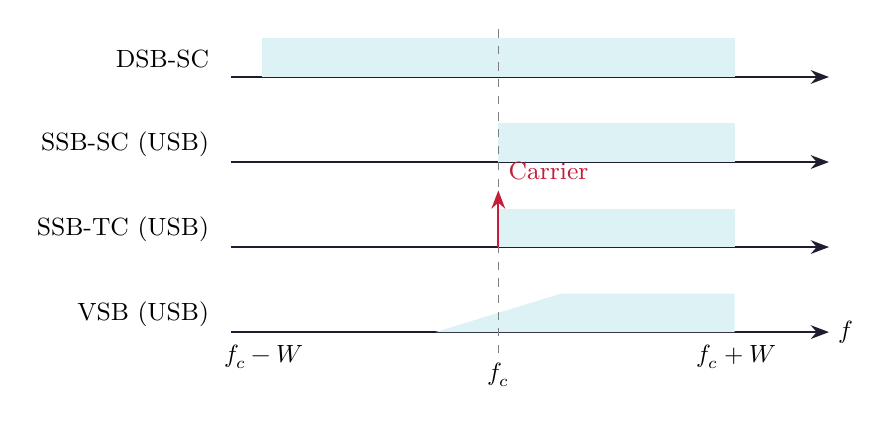
\begin{tikzpicture}[y=0.72cm,every node/.style={font=\small}]
 \foreach \y/\label in {5/DSB-SC,3.5/SSB-SC (USB),2/SSB-TC (USB),0.5/VSB (USB)}{
   \node[anchor=east] at (-3.55,\y+0.32) {\label};
   \draw[arrow] (-3.4,\y)--(4.2,\y);
 }
 \fill[hdrteal] (-3,5) rectangle (3,5.68);
 \fill[hdrteal] (0,3.5) rectangle (3,4.18);
 \fill[hdrteal] (0,2) rectangle (3,2.68);
 \fill[hdrteal] (-0.8,0.5)--(0.8,1.18)--(3,1.18)--(3,0.5)--cycle;
 \draw[dashed,gray] (0,0.13)--(0,5.86);
 \draw[redarrow] (0,2)--(0,3) node[above right] {\small Carrier};
 \node[below] at (-3,0.45) {$f_c-W$};
 \node[below] at (0,0.13) {$f_c$};
 \node[below] at (3,0.45) {$f_c+W$};
 \node[right] at (4.2,0.5) {$f$};
\end{tikzpicture}\par
\end{tcolorbox}


\subsection{Recovering the Baseband through a VSB Filter}
Consider the baseband-equivalent response of an ideal zero-phase RF filter. After filtering a DSB-SC signal, synchronous multiplication shifts the positive and negative RF bands back to baseband:
\[
\begin{aligned}
 S_D(f)&=\tfrac{A_c}{2}[M(f-f_c)+M(f+f_c)],\\
 Y(f)&=\tfrac{A_c}{2}M(f)\,[H(f+f_c)+H(f-f_c)],
       \qquad |f|\le W .
\end{aligned}
\]
This assumes a local oscillator of amplitude two and an ideal output low-pass filter. For a real, even response $H$, the two terms are $H(f_c+f)$ and $H(f_c-f)$. Their sum must be constant across the message band. Thus, near $f_c$, the decreasing response on one side complements the increasing response on the other. For unity target sum, $H(f_c)=1/2$. The spectrum sketch above shows occupied bands, while this condition explains why retaining a partial sideband can still give a flat recovered message.

\begin{tcolorbox}[examplebox, title={Check Complementary VSB Gain at Two Message Frequencies}]
Normalize the desired sum of the two VSB responses to one. At a $1\,\mathrm{kHz}$ offset, suppose the upper response is $0.82$ and the vestige response is $0.18$. At $3\,\mathrm{kHz}$ the full sideband has gain one and the vestige is zero.
\[
\begin{aligned}
 H(f_c+1\,\mathrm{kHz})+H(f_c-1\,\mathrm{kHz})&=0.82+0.18=1,\\
 H(f_c+3\,\mathrm{kHz})+H(f_c-3\,\mathrm{kHz})&=1+0=1.
\end{aligned}
\]
Both message components receive the same baseband gain $A_c/2$ in the chosen detector normalization. If the $1\,\mathrm{kHz}$ vestige is wrongly removed, that component falls to $0.82$ of its intended amplitude while the $3\,\mathrm{kHz}$ component stays the same.
\end{tcolorbox}

\newpage
\begin{center}
  {\large\bfseries\color{myred} Quick Revision --- Module 1}\\[3pt]
  {\small\color{mydark} Introduction and Continuous Wave Linear Modulation $|$ EC401}
\end{center}
\noindent{\color{myred}\rule{\linewidth}{1.2pt}}
\par\vspace{4pt}

\begin{tcolorbox}[formulabox, title={Key Formulas at a Glance}]
\renewcommand{\arraystretch}{1.35}
\noindent\begin{tabularx}{\linewidth}{B{4.4cm} Y}
Antenna length & $\ell=c/(4f)$ \\[4pt]
Conventional AM & $A_c(1+k_a m)\cos(2\pi f_ct)$ \\[4pt]
Tone sidebands & $f_c\pm f_m$, peak $\mu A_c/2$ each \\[4pt]
Envelope reading & $\mu=(E_{\max}-E_{\min})/(E_{\max}+E_{\min})$ \\[4pt]
Power and efficiency & $P_c=A_c^2/(2R)$ \newline $P_{\rm SB}=\mu^2P_c/2$ \quad $\eta=\mu^2/(2+\mu^2)$ \\[4pt]
DSB-SC power & $P_D=A_c^2\overline{m^2}/(2R)$ \\[4pt]
Bandwidth & DSB $2W$ \quad SSB $W$ \quad VSB $W+f_v$ \\[4pt]
\end{tabularx}\par
\end{tcolorbox}

\begin{tcolorbox}[defbox, title={One-Line Definitions}]
\begin{itemize}[leftmargin=*, itemsep=3pt, topsep=0pt]
  \item \textbf{Carrier.} A sinusoid used to position the message at RF.
  \item \textbf{Sideband.} A shifted part of the baseband spectrum carrying information.
  \item \textbf{Critical modulation.} The conventional AM envelope touches zero at $\mu=1$.
  \item \textbf{Vestige.} Part of the other sideband retained in VSB.
\end{itemize}
\end{tcolorbox}

\begin{tcolorbox}[exambox, title={Frequently Asked / Viva Questions}]
\begin{enumerate}[topsep=0pt, label=\textbf{Q\arabic*.}, itemsep=5pt]
  \item \Q{Why is modulation needed?}
    It enables practical antennas and places each signal in a suitable channel band.
  \item \Q{What do the transmitter and receiver do?}
    The transmitter prepares and launches the waveform. The receiver selects it and recovers the message.
  \item \Q{What are the AM lines for one tone?}
    $f_c$ and $f_c\pm f_m$, together with the negative-frequency mirrors.
  \item \Q{How do sideband phasors combine?}
    They rotate oppositely at $2\pi f_m$ in the carrier frame. In-phase projections add and transverse projections cancel.
  \item \Q{When is the envelope formula for modulation index valid?}
    When the magnitude envelope has no folding.
  \item \Q{What causes overmodulation distortion?}
    Negative portions of the signed envelope reverse RF phase. A magnitude detector folds them.
  \item \Q{What is the maximum single-tone conventional AM efficiency?}
    $1/3$ at $\mu=1$ for a nonfolded envelope.
  \item \Q{Why is DSB-SC received coherently?}
    The local reference preserves the sign of the message, which is lost in a magnitude detector.
  \item \Q{Does a transmitted SSB carrier increase bandwidth?}
    No. It adds a line at the existing band edge and increases power.
  \item \Q{Why is VSB useful near the carrier?}
    It relaxes the sharp transition required for SSB while keeping the bandwidth below full DSB.
\end{enumerate}
\end{tcolorbox}

\begin{tcolorbox}[tikzbox, unbreakable, title={Summary Comparison}]
\begingroup
\setlength{\tabcolsep}{5pt}
\setlength{\extrarowheight}{3pt}
\renewcommand{\arraystretch}{1.45}
\noindent\begin{tabularx}{\linewidth}{|B{3.35cm}|Y|Y|}
\hline
\multicolumn{1}{|c|}{\textbf{Scheme}} & \multicolumn{1}{c|}{\textbf{Transmitted components}} & \multicolumn{1}{c|}{\textbf{Bandwidth and use}} \\
\hline
DSB-TC & Carrier and both sidebands. & $2W$. Simple AM broadcast receivers. \\
\hline
DSB-SC & Both sidebands. & $2W$. Coherent reception. \\
\hline
SSB & One sideband, carrier optional. & $W$. Narrow voice channels. \\
\hline
VSB & Full sideband and vestige. & $W+f_v$. Analog video transmission. \\
\hline
\end{tabularx}\par
\endgroup
\end{tcolorbox}


% -- Module 2 -----------------------------------------------------------------
\modulestart{2}{Generation and Detection of Amplitude Modulation}

\section{Generation and Detection of Amplitude Modulation}
\subsection{Gated Modulator}
\begin{tcolorbox}[defbox, title={Carrier-Controlled Switching}]
A carrier-frequency switch gates a DC-biased message $u(t)=B+m(t)$. A band-pass filter (BPF) centred at $f_c$ selects the RF fundamental and its sidebands. For ideal half-duty gating $g(t)=1$ when $\cos(2\pi f_ct)>0$ and zero otherwise:
\[
\begin{aligned}
 g(t)&=\frac12+\frac{2}{\pi}\left[
 \cos(2\pi f_ct)-\frac13\cos(6\pi f_ct)+\cdots\right],\\
 v(t)&=[B+m(t)]g(t),\\
 s(t)&=\frac{2B}{\pi}\left[1+\frac{m(t)}{B}\right]\cos(2\pi f_ct).
\end{aligned}
\]
The BPF rejects baseband and harmonics. With $B=0$, the same ideal switch and filter produce DSB-SC from a zero-mean message. Real switching requires adequate carrier drive and filtering.
\end{tcolorbox}

\begin{tcolorbox}[tikzbox, unbreakable, title={Gated and Square-Law AM Generation}]
\centering
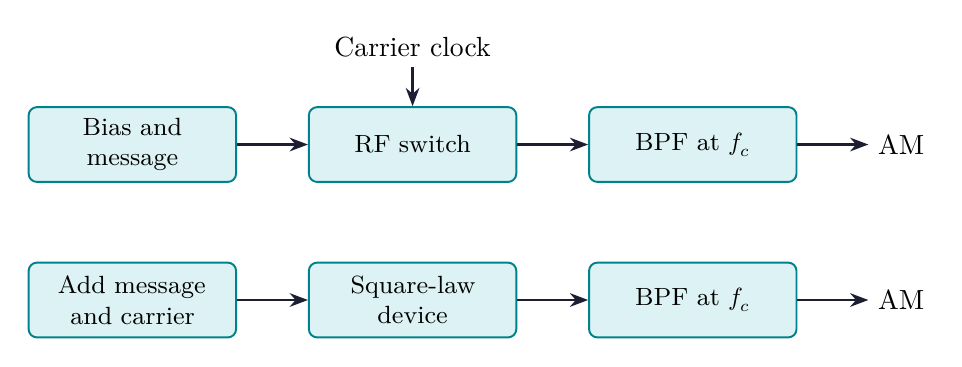
\begin{tikzpicture}[node distance=9mm]
  \node[block] (bias) {Bias and message};
  \node[block,right=of bias] (gate) {RF switch};
  \node[block,right=of gate] (bpf) {BPF at $f_c$};
  \node[right=9mm of bpf] (out) {AM};
  \draw[arrow] (bias)--(gate);
  \draw[arrow] (gate)--(bpf);
  \draw[arrow] (bpf)--(out);
  \node[above=5mm of gate] (osc) {Carrier clock};
  \draw[arrow] (osc)--(gate);
  \node[block,below=10mm of bias] (sum) {Add message and carrier};
  \node[block,right=of sum] (sq) {Square-law device};
  \node[block,right=of sq] (sel) {BPF at $f_c$};
  \node[right=9mm of sel] (out2) {AM};
  \draw[arrow] (sum)--(sq);
  \draw[arrow] (sq)--(sel);
  \draw[arrow] (sel)--(out2);
\end{tikzpicture}\par
\end{tcolorbox}

\subsection{Square-Law Modulator}
For a weakly nonlinear device $v_o=a_1v_i+a_2v_i^2$, let $v_i=m(t)+A\cos\omega_ct$. The coefficient $a_2$ has units $\mathrm{V^{-1}}$ for voltage in and out. Expand before filtering:
\[
\begin{aligned}
 v_o &= a_1m+a_1 A\cos\omega_ct+a_2m^2\\
     &\quad+2a_2Am\cos\omega_ct+a_2A^2\cos^2\omega_ct,\\
 s(t)&=a_1A\cos\omega_ct+2a_2Am(t)\cos\omega_ct\\
     &=a_1A\left[1+\frac{2a_2}{a_1}m(t)\right]\cos\omega_ct.
\end{aligned}
\]
The BPF removes $a_1m$, $a_2m^2$, DC and $2f_c$. This model assumes weak nonlinearity and a carrier well separated from the baseband harmonics.

\subsection{Balanced Modulator}
Two matched AM branches receive opposite message voltages and a common carrier. Subtracting their outputs cancels the carrier:
\[
\begin{aligned}
 u_+&=A_c(1+k_am)\cos\omega_ct,\quad
 u_-=A_c(1-k_am)\cos\omega_ct,\\
 s_D&=u_+-u_-\\
    &=2A_ck_a m(t)\cos\omega_ct.
\end{aligned}
\]
A transformer-coupled diode ring can implement balanced switching by reversing message polarity at the carrier rate. Mismatch leaves residual carrier. Balance and filtering set suppression in practice.

\begin{tcolorbox}[examplebox, title={Square-Law Modulator with a Specified Carrier and Tone}]
Let $v_o=2v_i+0.2v_i^2$, with the quadratic coefficient in $\mathrm{V^{-1}}$. The input combines a $4\,\mathrm V$ peak carrier and a $1.5\,\mathrm V$ peak message tone.
\[
\begin{aligned}
 A_{c,\rm out} &= a_1A=2(4)=8\,\mathrm V,\\
 k_a &= \frac{2a_2}{a_1}=\frac{2(0.2)}{2}=0.2\,\mathrm{V^{-1}},\\
 \mu&=k_aA_m=(0.2)(1.5)=0.30,\\
 A_{\rm USB}=A_{\rm LSB}&=\frac{\mu A_{c,\rm out}}2=1.2\,\mathrm V.
\end{aligned}
\]
The RF filter must pass both sidebands of the selected carrier and reject the terms around DC and $2f_c$. The result follows from the quadratic model. A practical circuit has higher-order terms and must limit its input swing.
\end{tcolorbox}

\subsection{Carrier Leakage in a Balanced Modulator}
If the lower branch has gain $g$ relative to the upper branch, the subtractor output is
\[
\begin{aligned}
 s(t) &= A_c[(1+k_am)-g(1-k_am)]\cos\omega_ct\\
      &= A_c(1-g)\cos\omega_ct
        +A_c(1+g)k_am(t)\cos\omega_ct.
\end{aligned}
\]
The first term is carrier leakage. For $g=0.98$ and $k_aA_m=0.5$, the leakage amplitude is $0.02A_c$. Each sideband has amplitude $(1.98)(0.5)A_c/2=0.495A_c$. The carrier is about $20\log_{10}(0.495/0.02)=27.9\,\mathrm{dB}$ below either sideband. Matching bias and gain reduces the leakage. Carrier suppression and sideband selection are separate design steps.

\section{Generation of Single Sideband}
\subsection{Filter Method}
Generate DSB-SC, pass only the desired sideband with a sharp BPF, and translate the retained band to its final channel if required. A message with lowest nonzero frequency $f_{\min}$ gives a gap of $2f_{\min}$ between the occupied bands. Little or no gap makes the filter difficult. Speech transmitters can limit low-frequency audio and first form SSB at a convenient IF.

\subsection{Phase-Shift Method}
Use a broadband $90^\circ$ message shifter to generate $\widehat m(t)$ and a carrier quadrature shifter to generate $\sin\omega_ct$. The balanced products are $m\cos\omega_ct$ and $\widehat m\sin\omega_ct$. Subtract for USB and add for LSB with this choice of phase:
\[
\begin{aligned}
 \cos\omega_mt\cos\omega_ct-\sin\omega_mt\sin\omega_ct
   &=\cos[(\omega_c+\omega_m)t],\\
 \cos\omega_mt\cos\omega_ct+\sin\omega_mt\sin\omega_ct
   &=\cos[(\omega_c-\omega_m)t].
\end{aligned}
\]
Gain or phase errors prevent complete cancellation. Maintaining a broadband quadrature shift is the main limitation.

\subsection{Third Method (Weaver)}
Weaver replaces the broadband audio phase shifter with two quadrature mixing stages and matched low-pass filters (LPFs). For an occupied message band $f_a$ to $f_b$, choose $f_0=(f_a+f_b)/2$. The first LPFs pass difference frequencies up to $(f_b-f_a)/2$. For a tone of peak $A_m$, let $\delta=2\pi(f_m-f_0)$:
\[
 I=\operatorname{LPF}[m\cos(2\pi f_0t)]
   =\frac{A_m}{2}\cos\delta t,\qquad
 Q=-\operatorname{LPF}[m\sin(2\pi f_0t)]
   =\frac{A_m}{2}\sin\delta t.
\]
The second stage combines $I\cos\omega_2t-Q\sin\omega_2t$ for USB with $f_2=f_c+f_0$, giving $f_2+(f_m-f_0)=f_c+f_m$. The sum gives the LSB if the second oscillator is set to $f_c-f_0$. Matched LPFs and quadrature oscillator accuracy determine image rejection.

\begin{tcolorbox}[tikzbox, unbreakable, title={Weaver Upper Sideband Signal Paths}]
\centering
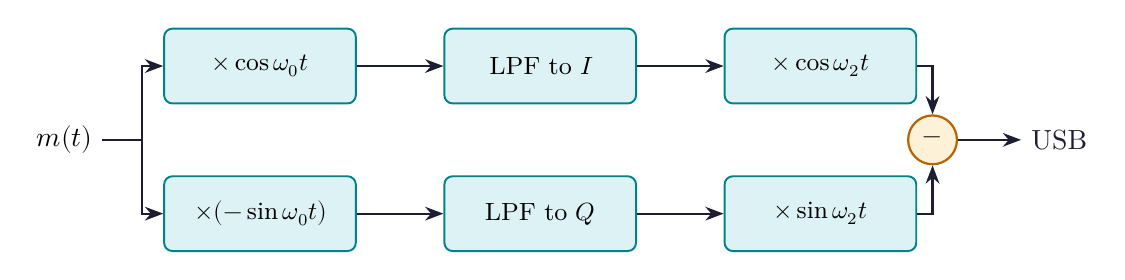
\begin{tikzpicture}[sblock/.style={block,text width=2.2cm},node distance=11mm]
  \node[sblock] (ic) {$\times\cos\omega_0t$};
  \node[sblock,below=9mm of ic] (qs) {$\times(-\sin\omega_0t)$};
  \node[sblock,right=of ic] (il) {LPF to $I$};
  \node[sblock,right=of qs] (ql) {LPF to $Q$};
  \node[sblock,right=of il] (mixi) {$\times\cos\omega_2t$};
  \node[sblock,right=of ql] (mixq) {$\times\sin\omega_2t$};
  \coordinate (mid) at ($(ic.center)!0.5!(qs.center)$);
  \node[left=20mm of mid] (in) {$m(t)$};
  \node[sumjunc,right=11mm of $(mixi.center)!0.5!(mixq.center)$] (sub) {$-$};
  \draw[arrow] (in.east)--++(5mm,0) |- (ic.west);
  \draw[arrow] (in.east)--++(5mm,0) |- (qs.west);
  \draw[arrow] (ic)--(il);
  \draw[arrow] (qs)--(ql);
  \draw[arrow] (il)--(mixi);
  \draw[arrow] (ql)--(mixq);
  \draw[arrow] (mixi.east)-| (sub.north);
  \draw[arrow] (mixq.east)-| (sub.south);
  \draw[arrow] (sub.east)--++(8mm,0) node[right] {USB};
\end{tikzpicture}\par
\end{tcolorbox}

\begin{tcolorbox}[examplebox, title={Weaver Frequency Plan for a Speech Channel}]
A voice channel spans $300$ to $2700\,\mathrm{Hz}$. Form USB on a $500\,\mathrm{kHz}$ nominal carrier.
\[
\begin{aligned}
 f_0&=\frac{300+2700}{2}=1500\,\mathrm{Hz},\\
 W_{\rm LP}&=\frac{2700-300}{2}=1200\,\mathrm{Hz},\\
 f_2&=f_c+f_0=501.5\,\mathrm{kHz}.
\end{aligned}
\]
After quadrature mixing and subtraction, the RF frequencies are $f_2+(f_m-f_0)$. A $900\,\mathrm{Hz}$ tone produces $500.9\,\mathrm{kHz}$, whereas $2400\,\mathrm{Hz}$ produces $502.4\,\mathrm{kHz}$. The occupied band is $500.3$--$502.7\,\mathrm{kHz}$. The negative difference frequency for $900\,\mathrm{Hz}$ is preserved by the quadrature paths.
\end{tcolorbox}

\subsection{Effect of Phase Error in the Phase-Shift Method}
For matched gains and an error $\delta$ in the relative quadrature phase, the two branch contributions at the wanted line add as $1+e^{j\delta}$. The unwanted line receives the difference $1-e^{j\delta}$. The amplitude leakage ratio is
\[
 \left|\frac{1-e^{j\delta}}{1+e^{j\delta}}\right|
   =\left|\tan\frac{\delta}{2}\right|.
\]
At a $5^\circ$ phase error, leakage is about $0.0437$ times the wanted line amplitude, or about $27.2\,\mathrm{dB}$ below it. A phase shifter that is accurate only at one audio frequency will give different rejection over the message band.

\section{Demodulation of Linear Modulation}
\subsection{AM Envelope Detector}
\begin{tcolorbox}[defbox, title={Diode Peak Detector}]
A diode charges $C$ near RF peaks, then blocks as the input falls. Between peaks, $C$ discharges through the load $R$. The smoothed voltage follows the envelope. A coupling capacitor or DC removal stage then recovers the audio. A large carrier, no envelope folding and a suitable $RC$ are required.
\end{tcolorbox}

\begin{tcolorbox}[tikzbox, unbreakable, title={Diode Envelope Detector Circuit}]
\centering
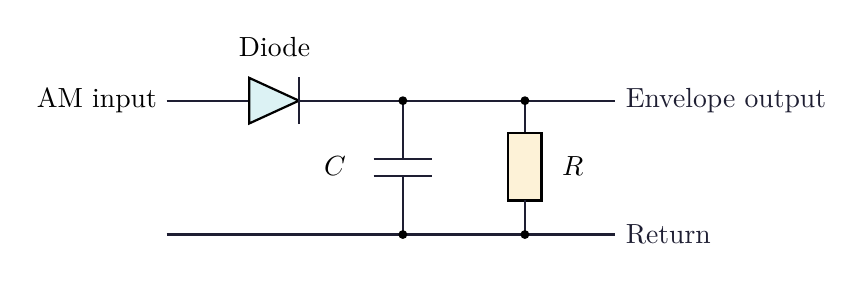
\begin{tikzpicture}[x=1cm,y=0.85cm]
  \node[left] at (0,2) {AM input};
  \draw[line] (0,2)--(1.05,2);
  \draw[fill=hdrteal,thick] (1.05,1.66)--(1.05,2.34)--(1.68,2)--cycle;
  \draw[line] (1.68,1.65)--(1.68,2.35);
  \draw[line] (1.68,2)--(5.7,2) node[right] {Envelope output};
  \node[above=4pt] at (1.37,2.35) {Diode};
  \draw[line] (0,0)--(5.7,0) node[right] {Return};
  \draw[line] (3,2)--(3,1.13);
  \draw[line] (2.63,1.13)--(3.37,1.13);
  \draw[line] (2.63,0.88)--(3.37,0.88);
  \draw[line] (3,0.88)--(3,0);
  \node[left=7pt] at (2.63,1.02) {$C$};
  \draw[line] (4.55,2)--(4.55,1.52);
  \draw[thick,fill=hdramber] (4.34,0.51) rectangle (4.76,1.52);
  \draw[line] (4.55,0.51)--(4.55,0);
  \node[right=4pt] at (4.76,1.02) {$R$};
  \foreach \x in {3,4.55}{\fill (\x,2) circle (1.6pt); \fill (\x,0) circle (1.6pt);}
\end{tikzpicture}\par
\end{tcolorbox}

Choose $RC$ long compared with the carrier period and short enough to follow the steepest envelope fall. Too short gives carrier ripple. Too long gives diagonal clipping. If $E(t)$ is the positive envelope, the ideal discharge slope just after a peak is $-E/RC$. On a falling part the discharge must be at least as steep:
\[
 RC\le \min_{\dot E<0}\frac{E(t)}{|\dot E(t)|}.
\]
With $E=A_c(1+\mu\cos\omega_mt)$, this ratio on the falling half-cycle is $(1+\mu\cos\theta)/(\mu\omega_m\sin\theta)$. Differentiating with respect to $\theta$ gives a stationary point at $\cos\theta=-\mu$. Therefore, for $0<\mu<1$,
\[
 \frac{1}{f_c}\ll RC
 \ \lesssim\ \frac{\sqrt{1-\mu^2}}{\mu\,2\pi f_m}.
\]
Real diode drop, source resistance and loading affect the actual design.

\begin{tcolorbox}[examplebox, title={Select a Detector Time Constant}]
Let $f_c=1\,\mathrm{MHz}$, $f_m=5\,\mathrm{kHz}$ and $\mu=0.6$.
\[
\begin{aligned}
 T_c &=1\,\mu\mathrm{s},\\
 RC_{\max}&=\frac{\sqrt{1-0.6^2}}{0.6(2\pi)(5000)}
            \approx42.4\,\mu\mathrm{s}.
\end{aligned}
\]
A starting choice is $R=10\,\mathrm{k}\Omega$ and $C=1.5\,\mathrm{nF}$, giving $RC=15\,\mu\mathrm{s}$. Check ripple and clipping at the worst specified modulation in the actual circuit.
\end{tcolorbox}

\subsection{Synchronous Detection and Mismatch}
Multiply $A_cm(t)\cos(2\pi f_ct)$ by $2\cos[2\pi(f_c+\Delta f)t+\phi]$ and low-pass filter:
\[
\begin{aligned}
 v(t)&=A_cm(t)\cos(2\pi\Delta ft+\phi)\\
     &\quad+A_cm(t)\cos[2\pi(2f_c+\Delta f)t+\phi],\\
 v_{\rm LP}(t)&=A_cm(t)\cos(2\pi\Delta ft+\phi).
\end{aligned}
\]
With only phase error, recovered amplitude scales by $\cos\phi$. At $90^\circ$ it vanishes. With frequency error the gain oscillates, causing beats and sign changes. A transmitted pilot can drive a carrier-recovery PLL. For DSB-SC without a pilot, a Costas loop or squaring loop can regenerate the reference. A recovered reference may retain a $180^\circ$ ambiguity, resolved by a known pilot or polarity reference. If RF filtering or the LPF removes part of a mismatch-shifted spectrum, the resulting waveform is additionally distorted.

\subsection{Carrier Recovery for DSB-SC: Squaring Loop and Costas Loop}
Because DSB-SC suppresses the carrier component completely, a coherent receiver must synthesize the carrier frequency and phase directly from the received sidebands. Two canonical circuits accomplish this:

\paragraph{1. Squaring Loop}
Passing $s(t)=A_cm(t)\cos(\omega_ct+\theta)$ through a square-law nonlinearity gives:
\[
s^2(t)=A_c^2m^2(t)\cos^2(\omega_ct+\theta)=\frac{1}{2}A_c^2m^2(t)\left[1+\cos(2\omega_ct+2\theta)\right].
\]
Since $m^2(t)\ge 0$ for all $t$, its expected value $\overline{m^2(t)}=P_m$ is strictly non-zero. A narrow bandpass filter (or PLL) centered at $2f_c$ extracts this discrete harmonic:
\[
v_{2f_c}(t)=\frac{1}{2}A_c^2P_m\cos(2\omega_ct+2\theta).
\]
Passing this signal through a frequency divider by two produces $\cos(\omega_ct+\theta)$ or $-\cos(\omega_ct+\theta)$, providing the coherent local reference with a $180^\circ$ phase ambiguity.

\paragraph{2. Costas Loop}
The Costas loop avoids RF frequency squaring by detecting the phase error directly at baseband through In-phase ($I$) and Quadrature ($Q$) channels:

\begin{tcolorbox}[tikzbox, unbreakable, title={Costas Loop Architecture for Coherent Carrier Recovery}]
\centering
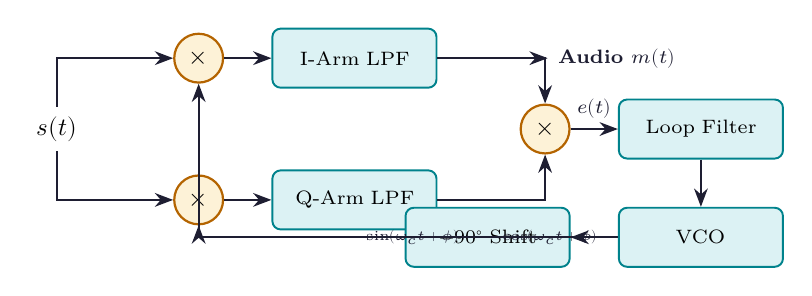
\begin{tikzpicture}[node distance=6mm, sblock/.style={block, text width=1.85cm, minimum height=0.75cm, font=\scriptsize}]
  \node (in) at (0,1.2) {\small $s(t)$};
  \node[sumjunc] (m1) at (1.8,2.1) {$\times$};
  \node[sumjunc] (m2) at (1.8,0.3) {$\times$};
  \node[sblock, right=of m1] (lpf1) {I-Arm LPF};
  \node[sblock, right=of m2] (lpf2) {Q-Arm LPF};
  \node[sumjunc] (m3) at (6.2,1.2) {$\times$};
  \node[sblock, right=of m3] (lf) {Loop Filter};
  \node[sblock, below=of lf] (vco) {VCO};
  \node[sblock, left=of vco] (ps) {$-90^\circ$ Shift};

  \draw[arrow] (in) |- (m1);
  \draw[arrow] (in) |- (m2);
  \draw[arrow] (m1) -- (lpf1);
  \draw[arrow] (m2) -- (lpf2);
  \draw[arrow] (lpf1.east) -| (m3.north);
  \draw[arrow] (lpf2.east) -| (m3.south);
  \draw[arrow] (m3) -- node[above] {\scriptsize $e(t)$} (lf);
  \draw[arrow] (lf) -- (vco);
  \draw[arrow] (vco) -- (ps);
  \draw[arrow] (vco.west) -| (m1.south) node[pos=0.15, right] {\tiny $\cos(\omega_c t+\phi)$};
  \draw[arrow] (ps.west) -| (m2.south) node[pos=0.15, right] {\tiny $-\sin(\omega_c t+\phi)$};
  \draw[arrow] (lpf1.east) -- ++(1.4,0) node[right] {\scriptsize \textbf{Audio $m(t)$}};
\end{tikzpicture}\par
\small When $\phi$ is small, the I-arm LPF yields $v_I(t)\approx\frac{A_c}{2}m(t)$ and the Q-arm LPF yields $v_Q(t)\approx\frac{A_c}{2}m(t)\phi$. Their product is $e(t)\approx\frac{A_c^2}{4}m^2(t)\phi$. Since $m^2(t)>0$, the loop filter integrates a DC error voltage strictly proportional to $\phi$, steering the VCO until $\phi\to 0$.
\end{tcolorbox}

\begin{tcolorbox}[examplebox, title={Frequency and Phase Error in a Coherent Receiver}]
For $m(t)=\cos(2\pi\,1000t)$, unit RF scale, and LO frequency offset $20\,\mathrm{Hz}$ with zero initial phase error, the detector yields
\[
 \begin{aligned}
 v_o(t)&=\cos(2\pi\,1000t)\cos(2\pi\,20t)\\
       &=\tfrac12\cos(2\pi\,1020t)+\tfrac12\cos(2\pi\,980t).
 \end{aligned}
\]
The two components bracket the original tone. With frequency lock restored but a constant $60^\circ$ phase error, the output instead becomes a single $1\,\mathrm{kHz}$ tone at half amplitude. Carrier phase and frequency recovery address different errors.
\end{tcolorbox}

\section{Superheterodyne Receiver}
Changing stations retunes the front end and local oscillator together so the wanted signal reaches the same intermediate-frequency filter.

\begin{tcolorbox}[defbox, title={Mix to a Fixed Intermediate Frequency}]
A tunable RF front end selects a station. The mixer shifts it to a fixed intermediate frequency (IF), where selectivity and gain are easier to implement. For the difference product,
\[
 f_{\rm IF}=|f_{\rm RF}-f_{\rm LO}|.
\]
The unwanted image lies on the opposite side of the LO from the desired RF. Both yield the same IF. The RF preselector must attenuate the image before mixing.
\end{tcolorbox}

\begin{tcolorbox}[tikzbox, unbreakable, title={Superheterodyne Receiver with RF Preselection and IF Filtering}]
\centering
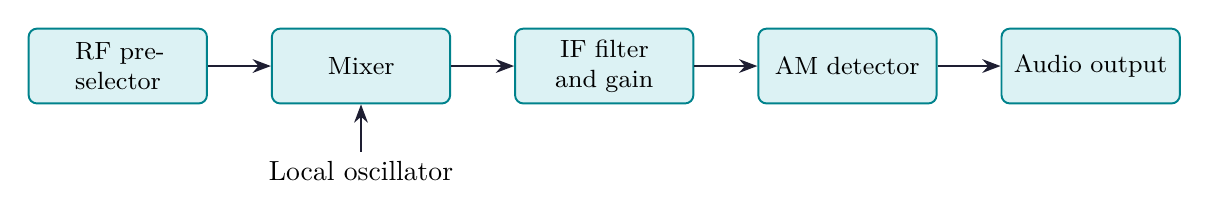
\begin{tikzpicture}[sblock/.style={block,text width=2.03cm},node distance=8mm]
  \node[sblock] (rf) {RF preselector};
  \node[sblock,right=of rf] (mix) {Mixer};
  \node[sblock,right=of mix] (if) {IF filter and gain};
  \node[sblock,right=of if] (det) {AM detector};
  \node[sblock,right=of det] (audio) {Audio output};
  \node[below=6mm of mix] (lo) {Local oscillator};
  \draw[arrow] (rf)--(mix);
  \draw[arrow] (mix)--(if);
  \draw[arrow] (if)--(det);
  \draw[arrow] (det)--(audio);
  \draw[arrow] (lo)--(mix);
\end{tikzpicture}\par
\end{tcolorbox}

\begin{tcolorbox}[formulabox, title={High-Side and Low-Side Injection}]
\[
\begin{aligned}
 \text{High-side:}\quad
 f_{\rm LO}&=f_{\rm RF}+f_{\rm IF}, & f_{\rm im}&=f_{\rm RF}+2f_{\rm IF},\\
 \text{Low-side:}\quad
 f_{\rm LO}&=f_{\rm RF}-f_{\rm IF}, & f_{\rm im}&=f_{\rm RF}-2f_{\rm IF}.
\end{aligned}
\]
The low-side image expression here assumes a positive physical RF image in the difference-mixing case. A larger IF separates the image further, while a lower IF can simplify sharp selectivity. Dual conversion can combine these benefits.
\end{tcolorbox}

\subsection{Receiver Selectivity before and after Mixing}
In high-side injection the wanted RF and the image lie below and above the LO, respectively. Taking the difference at the mixer maps both to the same IF. Increasing IF increases the $2f_{\rm IF}$ image separation. Tightening the RF preselector also improves image rejection, but it must still pass both wanted AM sidebands. The fixed IF filter sets adjacent-channel selectivity after conversion. Automatic gain control adjusts receiver gain as station strength varies.

\begin{tcolorbox}[tikzbox, unbreakable, title={Two RF Inputs Can Produce the Same Intermediate Frequency}]
\centering
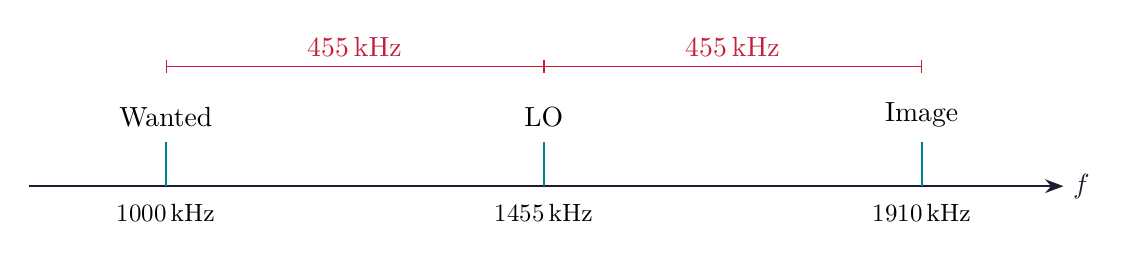
\begin{tikzpicture}[x=1.2cm,y=1cm]
 \draw[arrow] (-0.45,0)--(10.5,0) node[right] {$f$};
 \foreach \x/\f/\lab in {1/1000/Wanted,5/1455/LO,9/1910/Image}{
   \draw[myteal,thick] (\x,0)--(\x,0.56);
   \node[above=2pt] at (\x,0.56) {\lab};
   \node[below=3pt] at (\x,0) {\small $\f\,\mathrm{kHz}$};
 }
 \draw[|-|,myred] (1,1.52)--(5,1.52) node[midway,above] {$455\,\mathrm{kHz}$};
 \draw[|-|,myred] (5,1.52)--(9,1.52) node[midway,above] {$455\,\mathrm{kHz}$};
\end{tikzpicture}\par
\end{tcolorbox}

\begin{tcolorbox}[examplebox, title={Compute LO and Image Frequencies}]
For $f_{\rm RF}=1000\,\mathrm{kHz}$, $f_{\rm IF}=455\,\mathrm{kHz}$ and high-side injection,
\[
\begin{aligned}
 f_{\rm LO}&=1000+455=1455\,\mathrm{kHz},\\
 f_{\rm im}&=1455+455=1910\,\mathrm{kHz},\\
 |1910-1455|&=|1000-1455|=455\,\mathrm{kHz}.
\end{aligned}
\]
With low-side injection the LO is at $545\,\mathrm{kHz}$ and the corresponding image is at $90\,\mathrm{kHz}$. Both cases place the image $910\,\mathrm{kHz}$ from the desired station.
\end{tcolorbox}

\begin{tcolorbox}[examplebox, title={Calculate Image Rejection of a Single Tuned RF Stage}]
For an ideal single tuned preselector at $f_s$ with loaded quality factor $Q$, the normalized off-tune voltage gain is
\[
 \frac{|H(f)|}{|H(f_s)|}
 =\frac{1}{\sqrt{1+Q^2(f/f_s-f_s/f)^2}} .
\]
This form follows from the conductance and susceptance of a parallel RLC circuit. At $f_s=1\,\mathrm{MHz}$ with $Q=50$, compare high-side injection at two IFs:
\[
\begin{aligned}
 f_{\rm IF}=455\,\mathrm{kHz}:\quad f_{\rm im}&=1.910\,\mathrm{MHz},
 & |H(f_{\rm im})|/|H(f_s)|&\approx0.0144,\\[2pt]
 f_{\rm IF}=100\,\mathrm{kHz}:\quad f_{\rm im}&=1.200\,\mathrm{MHz},
 & |H(f_{\rm im})|/|H(f_s)|&\approx0.0545.
\end{aligned}
\]
The reductions are approximately $36.8$ and $25.3\,\mathrm{dB}$ respectively for equal antenna input voltages. A higher IF moves the image farther down the preselector response. The loaded bandwidth near resonance is about $f_s/Q=20\,\mathrm{kHz}$, so this example can still pass a $10\,\mathrm{kHz}$ wide AM channel.
\end{tcolorbox}

\newpage
\begin{center}
  {\large\bfseries\color{myred} Quick Revision --- Module 2}\\[3pt]
  {\small\color{mydark} AM and SSB Generation, Detection and Superheterodyne Reception $|$ EC401}
\end{center}
\noindent{\color{myred}\rule{\linewidth}{1.2pt}}
\par\vspace{4pt}

\begin{tcolorbox}[formulabox, title={Key Formulas at a Glance}]
\renewcommand{\arraystretch}{1.35}
\noindent\begin{tabularx}{\linewidth}{B{4.4cm} Y}
Gated AM & $\frac{2}{\pi}[B+m(t)]\cos(2\pi f_ct)$ \\[4pt]
Square-law AM & $k_a=2a_2/a_1$ after BPF \\[4pt]
Balanced output & $s_D=2A_ck_am(t)\cos\omega_ct$ \\[4pt]
Phase-shift SSB & $m\cos\omega_ct\mp\widehat m\sin\omega_ct$ \\[4pt]
Envelope detector & $1/f_c\ll RC\lesssim\sqrt{1-\mu^2}/(\mu\,2\pi f_m)$ \\[4pt]
Coherent mismatch & $v_{\rm LP}=A_cm(t)\cos(2\pi\Delta ft+\phi)$ \\[4pt]
IF and image & $f_{\rm IF}=|f_{\rm RF}-f_{\rm LO}|$ \newline $f_{\rm im}=f_{\rm RF}\pm2f_{\rm IF}$ for the indicated injection \\[4pt]
\end{tabularx}\par
\end{tcolorbox}

\begin{tcolorbox}[defbox, title={One-Line Definitions}]
\begin{itemize}[leftmargin=*, itemsep=3pt, topsep=0pt]
  \item \textbf{Balanced modulator.} A circuit that cancels the carrier and retains its product with the message.
  \item \textbf{Diagonal clipping.} Distortion when the detector cannot discharge fast enough to follow a falling envelope.
  \item \textbf{Image.} Unwanted RF frequency translated to the same IF as the desired station.
  \item \textbf{Coherent detection.} Product detection with a frequency- and phase-matched reference.
\end{itemize}
\end{tcolorbox}

\begin{tcolorbox}[exambox, title={Frequently Asked / Viva Questions}]
\begin{enumerate}[topsep=0pt, label=\textbf{Q\arabic*.}, itemsep=5pt]
  \item \Q{What selects the fundamental in a gated modulator?}
    An RF BPF at the switching frequency rejects the baseband and higher harmonic groups.
  \item \Q{Which square-law term creates sidebands?}
    The cross-product $2a_2Am\cos\omega_ct$.
  \item \Q{What causes residual carrier in a balanced modulator?}
    Gain, bias or phase mismatch prevents exact branch cancellation.
  \item \Q{What limits the filter method for SSB?}
    The transition near the carrier must fit the gap between the desired and undesired bands.
  \item \Q{How does Weaver avoid a broadband phase shifter?}
    Two quadrature mixers and matched LPFs form the needed components at low frequency.
  \item \Q{Why does an envelope detector need a suitable time constant?}
    It must suppress carrier ripple while tracking falling audio peaks.
  \item \Q{What is the effect of a phase error alone?}
    Baseband gain is multiplied by $\cos\phi$.
  \item \Q{How is a DSB-SC reference recovered?}
    A Costas loop or squaring loop can regenerate it. A polarity reference can resolve the possible $180^\circ$ ambiguity.
  \item \Q{Why use a fixed IF?}
    The receiver can use a fixed sharp filter and gain stage for different stations.
  \item \Q{Where is the image rejected?}
    In the RF preselector. The IF filter cannot distinguish it after conversion.
\end{enumerate}
\end{tcolorbox}

\begin{tcolorbox}[tikzbox, unbreakable, title={Summary Comparison}]
\begingroup
\setlength{\tabcolsep}{5pt}
\setlength{\extrarowheight}{3pt}
\renewcommand{\arraystretch}{1.45}
\noindent\begin{tabularx}{\linewidth}{|B{3.35cm}|Y|Y|}
\hline
\multicolumn{1}{|c|}{\textbf{Method}} & \multicolumn{1}{c|}{\textbf{Principle}} & \multicolumn{1}{c|}{\textbf{Design concern}} \\
\hline
Filter SSB & Reject one sideband of a DSB-SC signal. & Sharp transition near the carrier. \\
\hline
Phase-shift SSB & Cancel one band in quadrature. & Broadband phase accuracy. \\
\hline
Weaver SSB & Mix twice with quadrature oscillators and matched LPFs. & Branch matching and image rejection. \\
\hline
Envelope detector & Track a nonfolded AM envelope. & Ripple and diagonal clipping. \\
\hline
Synchronous detector & Mix with a locally regenerated carrier. & Frequency and phase lock. \\
\hline
\end{tabularx}\par
\endgroup
\end{tcolorbox}


% -- Module 3 -----------------------------------------------------------------
\modulestart{3}{Angle Modulation}

\section{Angle Modulation}
\subsection{Instantaneous Phase and Frequency}

\begin{tcolorbox}[defbox, title={FM and PM}]
An angle-modulated carrier has constant peak voltage $A_c$ and time-varying phase:
\[
\begin{aligned}
 s(t)&=A_c\cos[2\pi f_ct+\phi(t)],\\
 f_i(t)&=\frac{1}{2\pi}\frac{d}{dt}[2\pi f_ct+\phi(t)]
        =f_c+\frac{1}{2\pi}\frac{d\phi}{dt}.
\end{aligned}
\]
In frequency modulation (FM), $f_i-f_c=k_fm(t)$, where $k_f$ is in $\mathrm{Hz/V}$. In phase modulation (PM), $\phi=k_pm(t)$, with $k_p$ in $\mathrm{rad/V}$. An initial phase constant is absorbed into the carrier reference.
\end{tcolorbox}

\[
\begin{aligned}
 \phi_{\mathrm{FM}}(t)&=2\pi k_f\int_{t_0}^{t}m(\tau)\,d\tau,\\
 f_{i,\mathrm{PM}}(t)&=f_c+\frac{k_p}{2\pi}\frac{dm(t)}{dt}.
\end{aligned}
\]
An integrator followed by a phase modulator produces FM. A differentiator followed by a frequency modulator produces PM, with the appropriate gain and phase reference. Angle modulation keeps RF envelope power $A_c^2/(2R)$ constant. A receiver limiter can reject amplitude fluctuations before angular detection.

\subsection{Single-Tone Time-Domain Expressions}
Let $m(t)=A_m\cos(2\pi f_mt)$. Integrating or differentiating gives
\[
\begin{aligned}
 s_{\mathrm{FM}}(t)&=A_c\cos[\omega_ct+\beta\sin\omega_mt],
    &\beta&=\frac{\Delta f}{f_m}, & \Delta f&=k_fA_m,\\
 s_{\mathrm{PM}}(t)&=A_c\cos[\omega_ct+\beta_p\cos\omega_mt],
    &\beta_p&=k_pA_m, &\Delta f_{\mathrm{PM}}&=\beta_p f_m.
\end{aligned}
\]
Here $\omega=2\pi f$ and $\Delta f$ denotes the peak absolute frequency deviation in hertz. The dimensionless indices specify peak phase deviation in radians. At fixed message amplitude, increasing $f_m$ reduces the FM index, leaves the PM index fixed, and increases the frequency deviation of PM.

\begin{tcolorbox}[tikzbox, unbreakable, title={FM Becomes Denser Where Instantaneous Frequency Is Higher}]
\centering
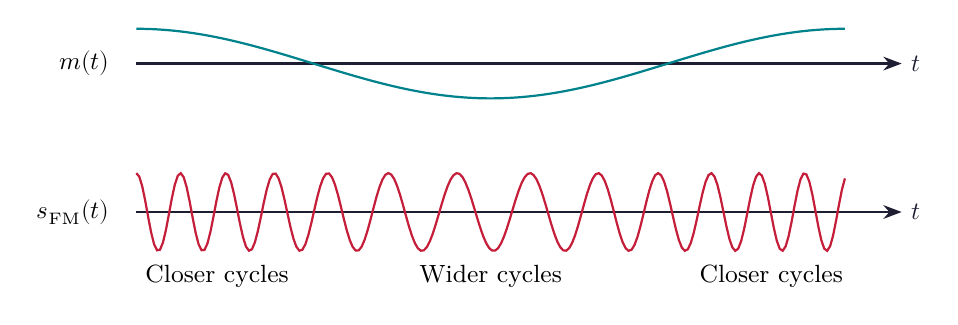
\begin{tikzpicture}[x=1.8cm,y=0.65cm,every node/.style={font=\small}]
  \draw[arrow] (0,2.9)--(5.4,2.9) node[right] {$t$};
  \draw[arrow] (0,0)--(5.4,0) node[right] {$t$};
  \draw[myteal,thick,domain=0:5,samples=100] plot (\x,{2.9+0.68*cos(72*\x)});
  \draw[myred,thick,domain=0:5,samples=240] plot (\x,{0.76*cos(930*\x+185*sin(72*\x))});
  \node[anchor=east] at (-0.12,2.9) {$m(t)$};
  \node[anchor=east] at (-0.12,0) {$s_{\rm FM}(t)$};
  \node[below] at (0.57,-0.85) {Closer cycles};
  \node[below] at (2.50,-0.85) {Wider cycles};
  \node[below] at (4.48,-0.85) {Closer cycles};
\end{tikzpicture}\par
\small Here $k_f>0$. The RF envelope remains constant at all three positions.
\end{tcolorbox}

\begin{tcolorbox}[examplebox, title={Compare FM and PM When the Message Frequency Doubles}]
Apply $m(t)=2\cos(2\pi\,2000t)\,\mathrm V$ to an FM modulator with $k_f=2\,\mathrm{kHz/V}$ and a PM modulator with $k_p=0.8\,\mathrm{rad/V}$.
\[
\begin{aligned}
 \Delta f_{\rm FM} &= k_f A_m=4\,\mathrm{kHz},\\
 \beta_{\rm FM}&=\Delta f_{\rm FM}/f_m=2,\\
 \beta_{\rm PM}&=k_pA_m=1.6,\\
 \Delta f_{\rm PM} &=\beta_{\rm PM}f_m=3.2\,\mathrm{kHz}.
\end{aligned}
\]
At $f_m=4\,\mathrm{kHz}$ with the same message peak, the FM deviation is still $4\,\mathrm{kHz}$ and its index becomes $1$. The PM index stays $1.6$ and its deviation rises to $6.4\,\mathrm{kHz}$. These are peak deviations. For the cosine message the FM frequency varies as a cosine, whereas in PM it varies as a negative sine from differentiating the phase.
\end{tcolorbox}

\section{Single-Tone Spectrum and Bessel Coefficients}
\subsection{Fourier Series Representation}
The complex factor $e^{j\beta\sin\omega_mt}$ is periodic at $f_m$. Its Fourier coefficient of order $n$ is a Bessel function of the first kind:
\[
\begin{aligned}
 J_n(\beta)&=\frac{1}{2\pi}\int_{-\pi}^{\pi}
            e^{j(\beta\sin\theta-n\theta)}\,d\theta,\\
 e^{j\beta\sin\omega_mt}&=\sum_{n=-\infty}^{\infty}
            J_n(\beta)e^{jn\omega_mt}.
\end{aligned}
\]
Multiply by $A_ce^{j\omega_ct}$ and take the real part:
\[
 s_{\rm FM}(t)=A_c\sum_{n=-\infty}^{\infty}
          J_n(\beta)\cos[(\omega_c+n\omega_m)t].
\]
The signed cosine coefficient is $A_cJ_n(\beta)$. In the two-sided Fourier transform, each cosine splits into two impulses of half this weight. Positive RF lines are drawn near $f_c$ for the orders of interest. A negative coefficient denotes a $\pi$ phase reversal, not negative power. Since $\cos\omega_mt=\sin(\omega_mt+\pi/2)$, single-tone PM obeys
\[
 s_{\rm PM}(t)=A_c\sum_{n=-\infty}^{\infty}
 J_n(\beta_p)\cos[(\omega_c+n\omega_m)t+n\pi/2].
\]
The complex weights of PM at the lines $f_c+nf_m$ are $A_cJ_n(\beta_p)e^{jn\pi/2}$ in the carrier-referenced representation. The positive-frequency Fourier impulse has half this weight and its negative-frequency image has the conjugate weight. At equal indices, the FM and PM magnitude spectra coincide. Their phases differ by $n\pi/2$ at the line of order $n$.

\begin{tcolorbox}[formulabox, title={Bessel Identities and Spectrum Power}]
\[
\begin{aligned}
 J_{-n}(\beta)&=(-1)^n J_n(\beta),\\
 J_0^2(\beta)+2\sum_{n=1}^{\infty}J_n^2(\beta)&=1,\\
 P_T&=P_c\left[J_0^2(\beta)+2\sum_{n=1}^{\infty}J_n^2(\beta)\right]
      =P_c,\qquad P_c=\frac{A_c^2}{2R}.
\end{aligned}
\]
Here $P_c$ denotes unmodulated carrier power. The line remaining at $f_c$ has power $P_c J_0^2(\beta)$. It vanishes at the first root $\beta\approx2.405$ while total RF power stays constant.
\end{tcolorbox}

\begin{tcolorbox}[tikzbox, unbreakable, title={FM and PM Line Magnitudes at Index One}]
\centering
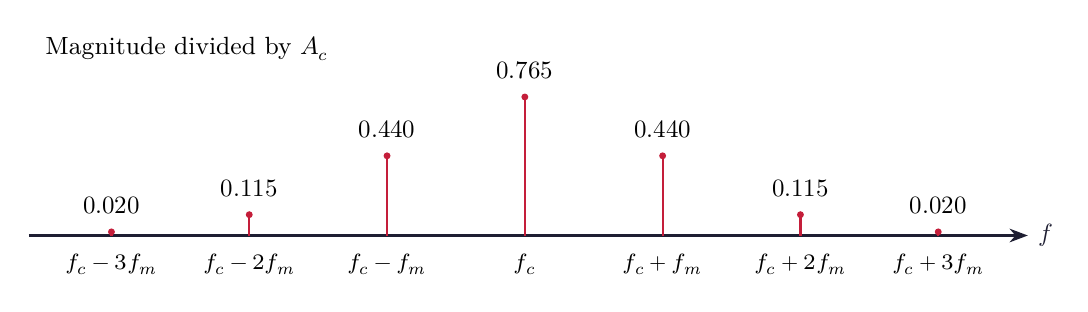
\begin{tikzpicture}[x=1.75cm,y=2.3cm,every node/.style={font=\small}]
  \draw[arrow] (-3.6,0)--(3.65,0) node[right] {$f$};
  \node[anchor=west] at (-3.55,1.03) {Magnitude divided by $A_c$};
  \foreach \n/\h/\v in {-3/0.020/0.020,-2/0.115/0.115,-1/0.440/0.440,0/0.765/0.765,1/0.440/0.440,2/0.115/0.115,3/0.020/0.020}{
    \draw[myred,thick] (\n,0)--(\n,\h);
    \fill[myred] (\n,\h) circle (1.25pt);
    \node[above=3pt] at (\n,\h) {$\v$};
  }
  \foreach \n/\ff in {-3/f_c-3f_m,-2/f_c-2f_m,-1/f_c-f_m,0/f_c,1/f_c+f_m,2/f_c+2f_m,3/f_c+3f_m}{
    \node[below=3pt] at (\n,0) {\footnotesize $\ff$};
  }
\end{tikzpicture}\par
\small For FM, the odd-order lower lines have reversed signs. For PM, apply the additional order-dependent $n\pi/2$ phase shift at the same index.
\end{tcolorbox}

\begin{tcolorbox}[examplebox, title={Calculate Carrier and Sideband Power from Bessel Coefficients}]
A constant-envelope FM carrier has peak $10\,\mathrm V$ across $50\,\Omega$, with $\beta=1$. The unmodulated carrier power is $1\,\mathrm W$. Using $J_0(1)\approx0.765198$, $J_1(1)\approx0.440051$ and $J_2(1)\approx0.114903$,
\[
\begin{aligned}
 P_{\rm carrier} &= P_cJ_0^2(1)\approx0.5855\,\mathrm W,\\
 P_{\pm1}\ \text{(each)} &=P_c J_1^2(1)\approx0.1936\,\mathrm W,\\
 P_{\pm2}\ \text{(each)} &=P_c J_2^2(1)\approx0.0132\,\mathrm W,\\
 P_{\text{through order 2}}
   &=P_{\rm carrier}+2P_{+1}+2P_{+2}\approx0.9992\,\mathrm W.
\end{aligned}
\]
The remaining power lies in the higher orders. Squaring the coefficient removes its sign for the power calculation. The same result holds for PM at index one because its additional line factors have unit magnitude.
\end{tcolorbox}

\subsection{Narrowband Approximation and Phasors}
If $|\phi(t)|\ll1$ rad, expand
\[
\begin{aligned}
 s(t)&=A_c[\cos\omega_ct\cos\phi(t)-\sin\omega_ct\sin\phi(t)]\\
     &\approx A_c\cos\omega_ct-A_c\phi(t)\sin\omega_ct.
\end{aligned}
\]
For tone FM, $J_0\approx1$ and $J_{\pm1}\approx\pm\beta/2$. For tone PM, the phase factors $e^{\pm j\pi/2}$ turn the first-order coefficients into $j\beta_p/2$ on both sides. The two sideband sums in the carrier frame are
\[
\begin{aligned}
 E_{\mathrm{SB,FM}}(t)
 &= \frac{A_c\beta}{2}\bigl(e^{j\omega_mt}-e^{-j\omega_mt}\bigr)\\
 &= jA_c\beta\sin\omega_mt,\\[3pt]
 E_{\mathrm{SB,PM}}(t)
 &= \frac{jA_c\beta_p}{2}\bigl(e^{j\omega_mt}+e^{-j\omega_mt}\bigr)\\
 &= jA_c\beta_p\cos\omega_mt.
\end{aligned}
\]
In both cases the sidebands add in quadrature to the carrier. For the cosine message, the PM phase swing is in step with the message and the FM phase swing is delayed by a quarter cycle. The baseband phase and frequency deviations follow the definitions above.

\begin{tcolorbox}[tikzbox, unbreakable, title={Narrowband FM and PM Phasor Construction}]
\centering
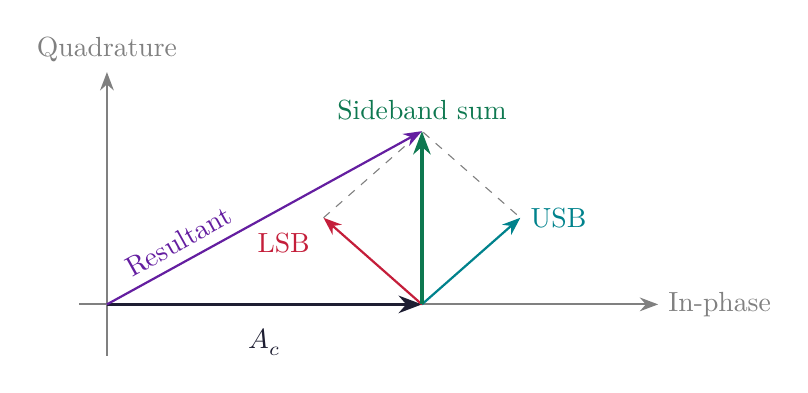
\begin{tikzpicture}
  \draw[arrow,gray] (-0.35,0)--(7,0) node[right] {In-phase};
  \draw[arrow,gray] (0,-0.65)--(0,2.95) node[above] {Quadrature};
  \draw[arrow,very thick] (0,0)--(4,0) node[midway,below=5pt] {$A_c$};
  \draw[arrow,thick,myteal] (4,0)--(5.25,1.1) node[right] {USB};
  \draw[redarrow,thick] (4,0)--(2.75,1.1);
  \node[myred,anchor=east] at (2.7,0.78) {LSB};
  \draw[dashed,gray] (2.75,1.1)--(4,2.2)--(5.25,1.1);
  \draw[arrow,mygreen,very thick] (4,0)--(4,2.2) node[above] {Sideband sum};
  \draw[arrow,mypurple,thick] (0,0)--(4,2.2);
  \node[above,rotate=29,mypurple] at (1.03,0.58) {Resultant};
\end{tikzpicture}\par
\small FM and PM share this geometry at a positive phase excursion. The sideband vectors for PM are the FM construction evaluated a quarter message period later, with the corresponding PM scale.
\end{tcolorbox}

\subsection{Wideband Angle Modulation and Carson's Rule}
When the phase deviation is not small, higher-order sidebands must be retained. The mathematical line spectrum has infinitely many orders. A useful occupied bandwidth estimate for message bandwidth $W$ and peak frequency deviation $\Delta f$ is
\[
 B_{\rm Carson}\approx 2(\Delta f+W)\quad(\mathrm{Hz}).
\]
For a tone put $W=f_m$. For PM with more than one tone, obtain $\Delta f$ from the peak of $|k_pm'(t)/(2\pi)|$. A narrowband first-order treatment gives approximately $2W$.

\begin{tcolorbox}[examplebox, title={Find Index, Line Positions and Bandwidth}]
The FM phase is $2\pi(100\times10^6)t+5\sin[2\pi(15\times10^3)t]$.
\[
\begin{aligned}
 f_c&=100\,\mathrm{MHz},& f_m&=15\,\mathrm{kHz},& \beta&=5,\\
 \Delta f&=\beta f_m=75\,\mathrm{kHz},\\
 B_{\rm Carson}&\approx 2(75+15)=180\,\mathrm{kHz}.
\end{aligned}
\]
The $n=\pm1$ lines lie at $99.985$ and $100.015\,\mathrm{MHz}$. Higher pairs are spaced by another $15\,\mathrm{kHz}$ per order. With a PM tone at the same frequency and peak phase deviation of $5$ rad, the magnitudes and Carson estimate are identical.
\end{tcolorbox}

\section{Generation of FM and PM}
\subsection{Direct FM with VCO or Reactance Modulator}
A voltage-controlled oscillator (VCO) tunes frequency through the applied voltage. Bias sets the unmodulated $f_c$. In its linear range $f_i=f_c+k_fm(t)$. A varactor changes tank capacitance. For inductance $L$ and total capacitance $C$,
\[
\begin{aligned}
 f_c &=\frac{1}{2\pi\sqrt{LC}},\\
 \Delta f&\approx-\frac{f_c}{2}\frac{\Delta C}{C}.
\end{aligned}
\]
The second line follows by differentiating $C^{-1/2}$ for a small capacitance swing. A reactance modulator makes a device draw a current approximately in quadrature with tank voltage. In one capacitive implementation $v_g\approx j\omega RC\,v$ and $i=g_m v_g$, so $i/v\approx j\omega g_mRC$. It behaves as $C_{\rm eff}\approx g_m RC$, tunable through transconductance $g_m$. A limiter stabilizes amplitude. Frequency drift and tuning nonlinearity limit direct FM unless controlled.

\subsection{Direct PM and Indirect FM (Armstrong)}
A quadrature phase modulator uses $\phi=k_pm(t)$ to control two gains, $I=\cos\phi$ and $Q=\sin\phi$. Weight the corresponding carrier branches and subtract:
\[
\begin{aligned}
 s(t)&=A_c[I\cos\omega_ct-Q\sin\omega_ct]\\
     &=A_c\cos(\omega_ct+\phi).
\end{aligned}
\]
For narrowband PM, use $I\approx1$ and $Q\approx\phi$ in the same structure. For wideband PM, use the full trigonometric gains so that $I^2+Q^2=1$ even at large phase deviation.

For indirect FM, integrate the message before the crystal-based narrowband phase modulator. The multiplier of factor $N$ multiplies $f_c$, the phase deviation and $\Delta f$ by $N$. A mixer with a fixed LO then sets the centre frequency without changing the magnitude of the deviation. This is the Armstrong route to wideband FM. The same multiplication chain can widen narrowband PM when the message integrator is bypassed.

\begin{tcolorbox}[tikzbox, unbreakable, title={Direct FM, Quadrature PM and Armstrong FM}]
\centering
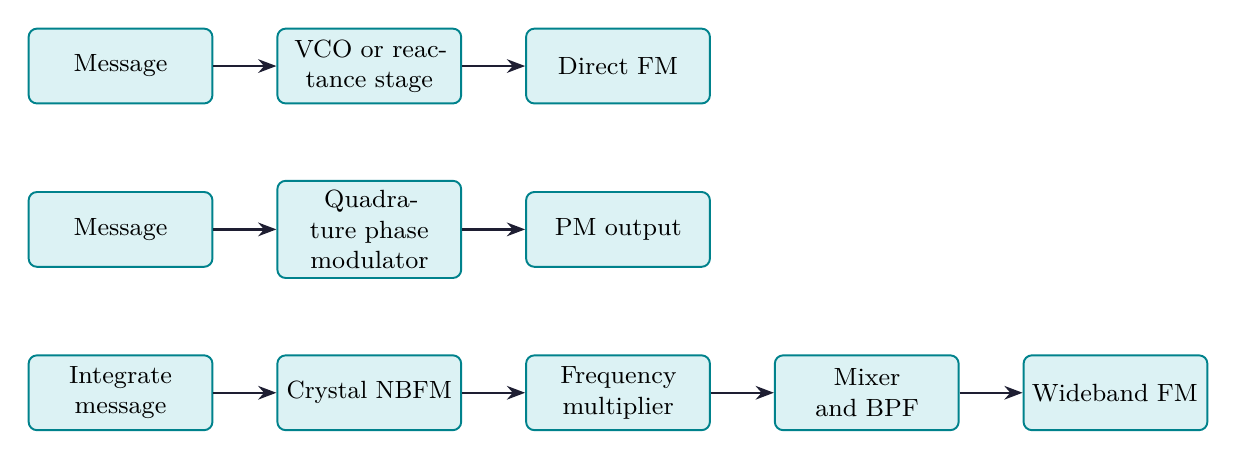
\begin{tikzpicture}[node distance=8mm,sblock/.style={block,text width=2.1cm}]
  \node[sblock] (m1) {Message};
  \node[sblock,right=of m1] (vco) {VCO or reactance stage};
  \node[sblock,right=of vco] (fm) {Direct FM};
  \draw[arrow] (m1)--(vco); \draw[arrow] (vco)--(fm);
  \node[sblock,below=11mm of m1] (m2) {Message};
  \node[sblock,right=of m2] (pm) {Quadrature phase modulator};
  \node[sblock,right=of pm] (pmo) {PM output};
  \draw[arrow] (m2)--(pm); \draw[arrow] (pm)--(pmo);
  \node[sblock,below=11mm of m2] (i) {Integrate message};
  \node[sblock,right=of i] (n) {Crystal NBFM};
  \node[sblock,right=of n] (mul) {Frequency multiplier};
  \node[sblock,right=of mul] (mix) {Mixer and BPF};
  \node[sblock,right=of mix] (out) {Wideband FM};
  \draw[arrow] (i)--(n); \draw[arrow] (n)--(mul);
  \draw[arrow] (mul)--(mix); \draw[arrow] (mix)--(out);
\end{tikzpicture}\par
\end{tcolorbox}

\begin{tcolorbox}[examplebox, title={Plan an Armstrong FM Channel}]
A stable $100\,\mathrm{kHz}$ narrowband source has $75\,\mathrm{Hz}$ peak deviation with a $3\,\mathrm{kHz}$ tone. The target is $100\,\mathrm{MHz}$ with $15\,\mathrm{kHz}$ peak deviation.
\[
\begin{aligned}
 \beta_{\rm seed} &= 75/3000=0.025,\\
 N &= \frac{15\,000}{75}=200,\\
 f_{\rm after\ multiplier}&=200(100\,\mathrm{kHz})=20\,\mathrm{MHz},\\
 \Delta f_{\rm after\ multiplier}&=200(75\,\mathrm{Hz})=15\,\mathrm{kHz}.
\end{aligned}
\]
Use an $80\,\mathrm{MHz}$ local oscillator and select the sum at $100\,\mathrm{MHz}$. Reject the unwanted difference product at $60\,\mathrm{MHz}$. The mixer changes the centre frequency and the target deviation remains $15\,\mathrm{kHz}$. The final tone index is $15/3=5$.
\end{tcolorbox}

\pagebreak[3]
\section{Demodulation of FM and PM}
\subsection{Frequency Discriminators: Slope, Balanced, Foster-Seeley and Ratio Detector}
A frequency discriminator produces an output voltage strictly proportional to the instantaneous frequency deviation: $v_d(t) \approx K_d[f_i(t)-f_c] \propto m(t)$. For PM, $v_d \propto m'(t)$, requiring post-detection integration to recover the original baseband message. The four canonical discriminator topologies are:

\begin{enumerate}[leftmargin=1.5em, itemsep=3pt]
  \item \textbf{Simple Slope Detector}: Uses a single parallel-tuned LC circuit tuned off-resonance ($f_0 \approx f_c + \delta f$). Operating along the slope of the resonance curve converts frequency swings into proportional envelope variations, rectified by an envelope detector. \textit{Drawback}: Highly non-linear transfer characteristic and severe susceptibility to input amplitude fluctuations.
  \item \textbf{Balanced Slope Detector (Round-Travis Circuit)}: Combines two tuned circuits staggered symmetrically at $f_c + \delta f$ and $f_c - \delta f$ with their rectified outputs connected in series opposition. The resulting S-curve cancels even-harmonic distortion and provides a linear response centered at $f_c$.
  \item \textbf{Foster-Seeley Discriminator}: Uses a double-tuned center-tapped transformer where primary voltage $V_p$ is coupled to the secondary center tap. At resonance ($f = f_c$), the secondary voltage $V_s$ is in exact quadrature ($90^\circ$ phase shift) with $V_p$. The diode voltages $|V_p + V_s/2|$ and $|V_p - V_s/2|$ are equal, yielding zero differential output. As frequency deviates, the phase shifts from $90^\circ$, producing a highly linear voltage proportional to $\Delta f$. However, output scales directly with input amplitude, requiring a prior limiter stage.
  \item \textbf{Ratio Detector}: Modifies the Foster-Seeley topology by reversing one diode and placing a large reservoir capacitor ($C_s \approx 10\,\mu\mathrm{F}$) across the load resistors. The large time constant ($R_LC_s \gg 1/f_m$) clamps the total voltage constant ($V_1 + V_2 = V_{\mathrm{const}}$). Fast amplitude fluctuations (such as ignition noise or multipath AM fading) cannot change this voltage, providing \textbf{inherent amplitude limiting} and eliminating the need for an external limiter stage.
\end{enumerate}

\par\vspace{6pt}\noindent
\begin{tabularx}{\linewidth}{|B{3.2cm}|Y|Y|Y|}
\hline
\rowcolor{hdrgray}
\textbf{Parameter} & \textbf{Balanced Slope} & \textbf{Foster-Seeley} & \textbf{Ratio Detector} \\
\hline
\textbf{Operating Principle} & Dual staggered LC slope conversion & Phase shift in center-tapped transformer & Phase shift with clamped sum voltage \\
\hline
\textbf{Linearity} & Moderate (limited linear skirt) & Excellent across wide deviation & Very good across linear S-curve \\
\hline
\textbf{Limiter Requirement} & Mandatory (sensitive to AM noise) & Mandatory (output $\propto$ RF amplitude) & \textbf{Not Required} (inherent AM suppression) \\
\hline
\textbf{Alignment Complexity}& High (three distinct tuned frequencies) & Moderate (both tuned to exact $f_c$) & Moderate (both tuned to exact $f_c$) \\
\hline
\textbf{Primary Application}& Low-cost communication receivers & High-fidelity FM test instrumentation & Standard commercial broadcast FM receivers \\
\hline
\end{tabularx}
\par\vspace{12pt}

\begin{tcolorbox}[tikzbox, unbreakable, title={Balanced Frequency Discriminator}]
\centering
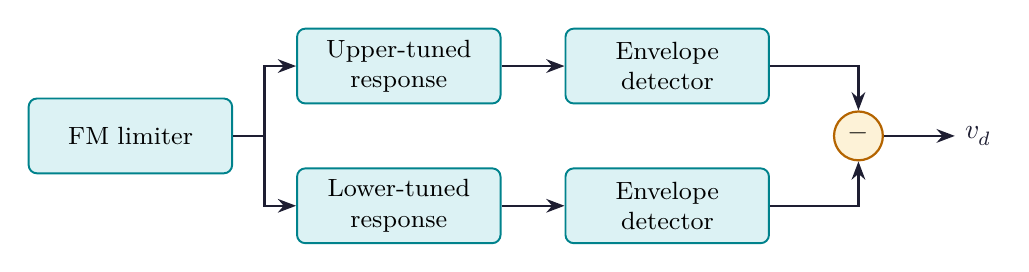
\begin{tikzpicture}[node distance=8mm,sblock/.style={block,text width=2.35cm}]
  \node[sblock] (hi) {Upper-tuned response};
  \node[sblock,below=8mm of hi] (lo) {Lower-tuned response};
  \node[sblock,right=of hi] (dh) {Envelope detector};
  \node[sblock,right=of lo] (dl) {Envelope detector};
  \coordinate (leftmid) at ($(hi.west)!0.5!(lo.west)$);
  \node[sblock,left=of leftmid] (lim) {FM limiter};
  \coordinate (rightmid) at ($(dh.east)!0.5!(dl.east)$);
  \node[sumjunc,right=of rightmid] (sub) {$-$};
  \draw[arrow] (lim.east)--++(4mm,0)|-(hi.west);
  \draw[arrow] (lim.east)--++(4mm,0)|-(lo.west);
  \draw[arrow] (hi)--(dh);
  \draw[arrow] (lo)--(dl);
  \draw[arrow] (dh.east)-|(sub.north);
  \draw[arrow] (dl.east)-|(sub.south);
  \draw[arrow] (sub.east)--++(9mm,0) node[right] {$v_d$};
\end{tikzpicture}\par
\small The two envelopes are equal at the centre frequency. Above centre the upper branch dominates, and below centre the lower branch dominates.
\end{tcolorbox}

\subsection{Phase-Locked Loop}
A PLL compares the input and VCO phases, filters the phase error, and drives the VCO to track the input. For a linearized phase detector with gain $K_p$ in $\mathrm{V/rad}$ and VCO gain $K_v$ in $\mathrm{Hz/V}$:
\[
 v_e=K_p(\theta_i-\theta_o),\qquad
 f_{\rm VCO}=f_{\rm free}+K_vv_{\rm ctrl}.
\]
When locked and tracking sufficiently fast, with $f_{\rm free}=f_c$,
\[
 v_{\rm ctrl}\approx\frac{f_i-f_c}{K_v}
                  =\frac{k_f}{K_v}m(t)\quad\text{for FM}.
\]
The control voltage yields the time derivative of the phase deviation for PM. Integration recovers that phase up to a reference constant. Capture means acquiring lock from an unlocked state. The lock range describes how far frequency may move after lock is established. Loop bandwidth trades tracking against noise rejection.

\begin{tcolorbox}[tikzbox, unbreakable, title={PLL Feedback and Demodulated Output}]
\centering
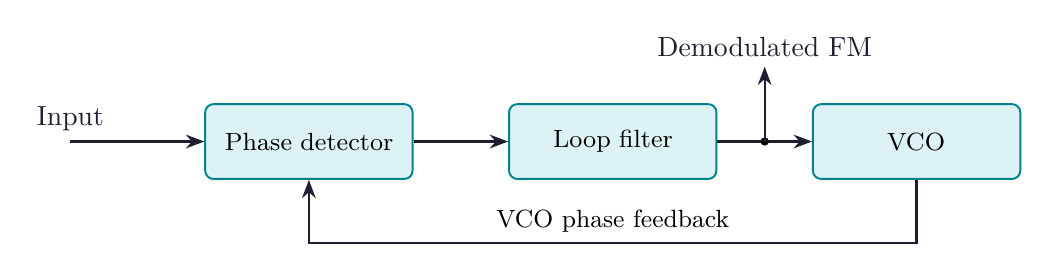
\begin{tikzpicture}[node distance=12mm]
  \node[block] (pd) {Phase detector};
  \node[block,right=of pd] (lf) {Loop filter};
  \node[block,right=of lf] (vco) {VCO};
  \draw[arrow] ([xshift=-17mm]pd.west)--(pd.west) node[pos=0,above] {Input};
  \draw[arrow] (pd)--(lf);
  \draw[arrow] (lf)--(vco);
  \coordinate (tap) at ($(lf.east)!0.5!(vco.west)$);
  \fill (tap) circle (1.5pt);
  \draw[arrow] (tap)--++(0,0.95) node[above] {Demodulated FM};
  \draw[arrow] (vco.south)--++(0,-0.8)-| (pd.south);
  \node at ($(lf.south)+(0,-0.52)$) {\small VCO phase feedback};
\end{tikzpicture}\par
\end{tcolorbox}

\begin{samepage}
\subsection{Why a Locked PLL Tracks Only within Its Loop Bandwidth}
For an ideal first-order model, replace the loop filter by a constant gain $K_L$ in the frequency range being analysed. Let $\Theta_i(s)$ and $\Theta_o(s)$ be the Laplace transforms of the input and oscillator phase deviations. The VCO integrates the frequency change to produce phase, so
\[
\begin{aligned}
 V_{\rm ctrl}(s)&=K_LK_p[\Theta_i(s)-\Theta_o(s)],\\
 s\Theta_o(s)&=2\pi K_v V_{\rm ctrl}(s),\\
 \frac{\Theta_o(s)}{\Theta_i(s)}
   &=\frac{K}{s+K},\qquad K=2\pi K_vK_LK_p .
\end{aligned}
\]
Here $K_p$ is the detector gain in $\mathrm{V/rad}$, $K_v$ is VCO sensitivity in $\mathrm{Hz/V}$, and $K$ is in $\mathrm{s^{-1}}$. With positive loop gain, the response is close to unity for angular modulation frequencies much smaller than $K$. A practical loop filter changes this transfer function. This small-signal result describes tracking after acquisition. Capture and lock range require the nonlinear loop behaviour.
\par
\end{samepage}

\begin{tcolorbox}[examplebox, title={Demodulate FM with a Locked PLL}]
Let $A_m=2\,\mathrm V$, $k_f=15\,\mathrm{kHz/V}$, $K_v=20\,\mathrm{kHz/V}$ and $f_{\rm free}=f_c$.
\[
\begin{aligned}
 \Delta f &= k_fA_m=30\,\mathrm{kHz},\\
 V_{\rm ctrl,peak} &\approx \frac{\Delta f}{K_v}=1.5\,\mathrm V.
\end{aligned}
\]
A gain of $4/3$ restores the original voltage scale while the PLL stays locked and tracks the tone.
\end{tcolorbox}

\begin{tcolorbox}[examplebox, title={Check PLL Tracking for Two Audio Frequencies}]
In the first-order model, let $K=2\pi(5000)\,\mathrm{s^{-1}}$. For an input phase tone of frequency $f_m$ the gain and phase lag of the tracked phase are
\[
 \left|\frac{\Theta_o}{\Theta_i}\right|
    =\frac{1}{\sqrt{1+(2\pi f_m/K)^2}},\qquad
 \angle\frac{\Theta_o}{\Theta_i}=-\tan^{-1}(2\pi f_m/K).
\]
At $1\,\mathrm{kHz}$ the ratio $2\pi f_m/K$ is $0.2$, so the tracked phase has gain $0.981$ and lag $11.3^\circ$. At $10\,\mathrm{kHz}$ the ratio is $2$, so gain falls to $0.447$ and lag rises to $63.4^\circ$. The second case illustrates attenuation and phase lag while locked. It does not by itself predict loss of lock.
\end{tcolorbox}

\newpage
\begin{center}
  {\large\bfseries\color{myred} Quick Revision --- Module 3}\\[3pt]
  {\small\color{mydark} Angle Modulation, Generation and Demodulation $|$ EC401}
\end{center}
\noindent{\color{myred}\rule{\linewidth}{1.2pt}}
\par\vspace{4pt}

\begin{tcolorbox}[formulabox, title={Key Formulas at a Glance}]
\renewcommand{\arraystretch}{1.35}
\noindent\begin{tabularx}{\linewidth}{B{4.4cm} Y}
Instantaneous frequency & $f_i=f_c+\phi'(t)/(2\pi)$ \\[4pt]
FM and PM phase & $\phi_{\rm FM}=2\pi k_f\int m(t)\,dt$ \newline $\phi_{\rm PM}=k_pm(t)$ \\[4pt]
Single-tone indices & $\beta=\Delta f/f_m$ for FM \quad $\beta_p=k_pA_m$ for PM \\[4pt]
Bessel spectrum & Tone lines at $f_c+nf_m$ \newline FM cosine coefficient $A_cJ_n(\beta)$ \\[4pt]
Carson estimate & $B\approx 2(\Delta f+W)$ \\[4pt]
Frequency multiplication & $f_c,\Delta f,\beta$ multiply by $N$ for tone FM \\[4pt]
FM detection & $v_d\approx K_d(f_i-f_c)$ \newline $v_{\rm ctrl}\approx(f_i-f_c)/K_v$ while tracking in lock \\[4pt]
\end{tabularx}\par
\end{tcolorbox}

\begin{tcolorbox}[defbox, title={One-Line Definitions}]
\begin{itemize}[leftmargin=*, itemsep=3pt, topsep=0pt]
  \item \textbf{Deviation.} Peak magnitude of $f_i-f_c$ in hertz.
  \item \textbf{Bessel coefficient.} Fourier-series coefficient of the single-tone angle-modulation factor.
  \item \textbf{Discriminator.} Converts instantaneous frequency offset to voltage.
  \item \textbf{PLL.} Feedback loop that tracks the input carrier phase.
\end{itemize}
\end{tcolorbox}

\begin{tcolorbox}[exambox, title={Frequently Asked / Viva Questions}]
\begin{enumerate}[topsep=0pt, label=\textbf{Q\arabic*.}, itemsep=5pt]
  \item \Q{Which carrier property stays constant?}
    Peak amplitude stays constant in ideal FM and PM.
  \item \Q{How can a PM circuit generate FM?}
    Integrate the message before applying it to the phase modulator.
  \item \Q{What happens to the PM frequency deviation as tone frequency increases?}
    It increases as $\Delta f_{\rm PM}=k_pA_mf_m$ for fixed amplitude.
  \item \Q{Why can the FM carrier line disappear?}
    $J_0(\beta)$ can be zero. The power is redistributed among sidebands.
  \item \Q{What does a negative Bessel coefficient mean?}
    A $\pi$ phase reversal of that cosine component. Its contribution to power stays positive.
  \item \Q{Why is the NBFM sideband sum in quadrature?}
    The opposite signed first-order coefficients cancel the horizontal projections and add the vertical ones.
  \item \Q{Why use a multiplier in Armstrong FM?}
    It increases the deviation of a stable narrowband source. A mixer then sets the desired channel centre.
  \item \Q{How does a reactance modulator tune FM?}
    A control voltage varies the effective reactive admittance of the oscillator tank.
  \item \Q{How does a discriminator recover PM?}
    Its output is proportional to the message derivative. Integrate to recover the original message up to a reference constant.
  \item \Q{What makes the PLL control voltage useful for FM?}
    While locked and tracking, it supplies the VCO frequency correction and is proportional to $m(t)$.
\end{enumerate}
\end{tcolorbox}

\begin{tcolorbox}[tikzbox, unbreakable, title={Summary Comparison}]
\begingroup
\setlength{\tabcolsep}{5pt}
\setlength{\extrarowheight}{3pt}
\renewcommand{\arraystretch}{1.45}
\noindent\begin{tabularx}{\linewidth}{|B{3.35cm}|Y|Y|}
\hline
\multicolumn{1}{|c|}{\textbf{Feature}} & \multicolumn{1}{c|}{\textbf{Frequency modulation}} & \multicolumn{1}{c|}{\textbf{Phase modulation}} \\
\hline
Directly controlled & $f_i-f_c=k_fm(t)$ & $\phi=k_pm(t)$ \\
\hline
Tone frequency deviation & $k_fA_m$ & $k_pA_m f_m$ \\
\hline
Before alternate modulator & Integrate before PM. & Differentiate before FM. \\
\hline
After discriminator & Scale directly. & Integrate and scale. \\
\hline
\end{tabularx}\par
\endgroup
\end{tcolorbox}


% -- Module 4 -----------------------------------------------------------------
\modulestart{4}{Multiplexing and Stereo Transmission}

\section{Multiplexing and Stereo Transmission}
\subsection{Frequency Division Multiplexing}
\begin{tcolorbox}[defbox, title={FDM}]
Frequency division multiplexing translates each input to a distinct frequency band and adds the bands for simultaneous transmission. At the receiver, BPFs select the desired bands before demodulation. Guard bands allow realizable filter transitions and reduce adjacent-channel interference.
\end{tcolorbox}
If $N$ equal-width channels each occupy $B_{\rm ch}$ and adjacent channels have guard $g$, the span from the first occupied edge to the last is
\[
 B_{\rm span}=NB_{\rm ch}+(N-1)g.
\]
For four $3\,\mathrm{kHz}$ SSB channels with $1\,\mathrm{kHz}$ internal guards, this gives $4(3)+3(1)=15\,\mathrm{kHz}$. External allocation margins, if specified, must be added separately.

\begin{tcolorbox}[tikzbox, unbreakable, title={FDM Channels and Guard Bands}]
\centering
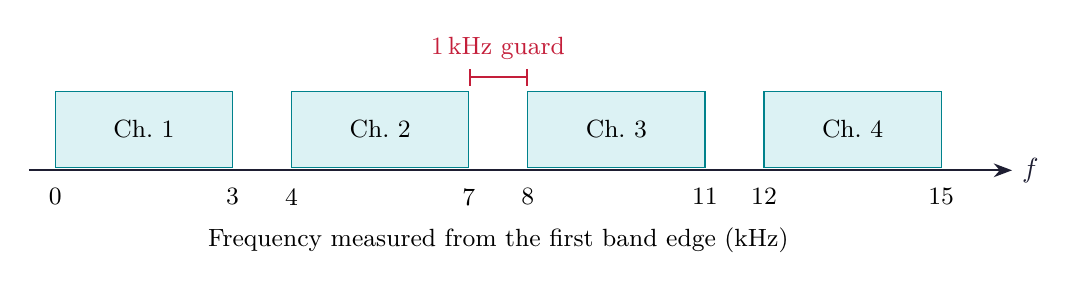
\begin{tikzpicture}[x=0.75cm]
  \draw[arrow] (-0.45,0)--(16.2,0) node[right] {$f$};
  \foreach \a/\b/\ch in {0/3/1,4/7/2,8/11/3,12/15/4}{
    \filldraw[fill=hdrteal,draw=myteal] (\a,0.04) rectangle (\b,1);
    \node at ({(\a+\b)/2},0.52) {\small Ch.\ \ch};
    \node[below=3pt] at (\a,0) {\small \a};
    \node[below=3pt] at (\b,0) {\small \b};
  }
  \draw[|-|,myred,thick] (7,1.18)--(8,1.18);
  \node[above=3pt,myred] at (7.5,1.18) {\small $1\,\mathrm{kHz}$ guard};
  \node[below] at (7.5,-0.6) {\small Frequency measured from the first band edge (kHz)};
\end{tikzpicture}\par
\end{tcolorbox}

\subsection{Time Division Multiplexing}
\begin{tcolorbox}[defbox, title={Synchronous TDM}]
Time division multiplexing assigns successive time slots to different inputs. In analog PAM-TDM, a clocked commutator samples each band-limited input once per frame. A synchronized receiver routes slots back to their channels and reconstruction LPFs recover the messages.
\end{tcolorbox}
For equal channel bandwidth $W$, each frame must recur at $f_s\ge 2W$ in the ideal sampling model. With $N$ equal slots and $n_{\rm ov}$ additional synchronization slots per frame,
\[
 R_{\rm slot}=(N+n_{\rm ov})f_s,\qquad
 T_{\rm slot}=\frac{1}{R_{\rm slot}}.
\]
Three channels limited to $3\,\mathrm{kHz}$ can be sampled at $8\,\mathrm{kHz}$ each. With one framing slot, the aggregate is $32\,\mathrm{kslot/s}$ and each slot is $31.25\,\mu\mathrm{s}$. Pulse shape, guard time and filtering determine required channel bandwidth. The slot rate alone does not specify it.

\begin{tcolorbox}[tikzbox, unbreakable, title={Two Frames of Three-Channel TDM}]
\centering
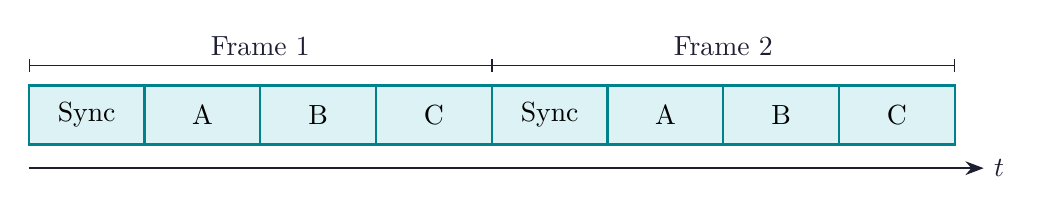
\begin{tikzpicture}[x=1.47cm]
  \foreach \x/\lab in {0/Sync,1/A,2/B,3/C,4/Sync,5/A,6/B,7/C}{
    \draw[thick,draw=myteal,fill=hdrteal] (\x,0) rectangle ++(1,0.75);
    \node at (\x+0.5,0.38) {\lab};
  }
  \draw[|-|,mydark] (0,1)--(4,1) node[midway,above] {Frame 1};
  \draw[|-|,mydark] (4,1)--(8,1) node[midway,above] {Frame 2};
  \draw[arrow] (0,-0.3)--(8.25,-0.3) node[right] {$t$};
\end{tikzpicture}\par
\end{tcolorbox}

FDM requires separate frequency slots and filter selectivity. TDM needs sample timing and frame synchronization. FDM is used in broadcast channel allocation and multicarrier links. TDM is used in shared sampled-data and telephone links.

\subsection{FM Stereo}
Form the sum $S=L+R$ and difference $D=L-R$. A pilot-tone stereo multiplex carries $S$ in the $0$--$15\,\mathrm{kHz}$ band, a $19\,\mathrm{kHz}$ pilot, and DSB-SC $D$ around $38\,\mathrm{kHz}$, occupying $23$--$53\,\mathrm{kHz}$. This composite controls the FM transmitter. A mono receiver recovers the low-pass sum. A stereo receiver locks to the pilot, regenerates the $38\,\mathrm{kHz}$ subcarrier, coherently detects $D$, and reconstructs
\[
 L=\frac{S+D}{2},\qquad R=\frac{S-D}{2}.
\]
Pilot recovery and matched audio paths maintain stereo separation. Without a usable pilot the receiver can fall back to mono.

\begin{tcolorbox}[tikzbox, unbreakable, title={FM Stereo Encoder and Decoder}]
\centering
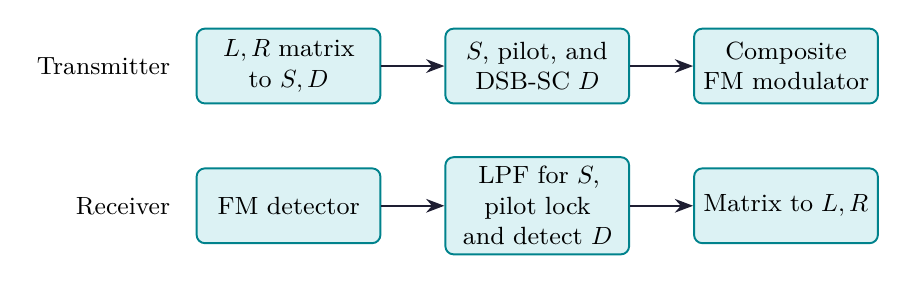
\begin{tikzpicture}[node distance=8mm,sblock/.style={block,text width=2.1cm}]
  \node[sblock] (m) {$L,R$ matrix to $S,D$};
  \node[sblock,right=of m] (c) {$S$, pilot, and DSB-SC $D$};
  \node[sblock,right=of c] (t) {Composite FM modulator};
  \draw[arrow] (m)--(c); \draw[arrow] (c)--(t);
  \node[sblock,below=8mm of m] (r) {FM detector};
  \node[sblock,right=of r] (d) {LPF for $S$, pilot lock and detect $D$};
  \node[sblock,right=of d] (o) {Matrix to $L,R$};
  \draw[arrow] (r)--(d); \draw[arrow] (d)--(o);
  \node[anchor=east] at ([xshift=-2mm]m.west) {\small Transmitter};
  \node[anchor=east] at ([xshift=-2mm]r.west) {\small Receiver};
\end{tikzpicture}\par
\end{tcolorbox}

\begin{tcolorbox}[examplebox, title={Trace and Recover the FM Stereo Channels}]
A left-only $8\,\mathrm{kHz}$ tone $L(t)$ enters the encoder, with $R(t)=0$. The sum and difference signals both equal $L(t)$.
\begin{itemize}[leftmargin=*, itemsep=3pt]
 \item The sum occupies baseband at $8\,\mathrm{kHz}$. A mono receiver passes it directly.
 \item The difference modulates the suppressed $38\,\mathrm{kHz}$ subcarrier. Its two lines lie at $30$ and $46\,\mathrm{kHz}$. A pilot at $19\,\mathrm{kHz}$ supplies the receiver's phase reference.
 \item After product detection and low-pass filtering, the decoder obtains $S=D=L(t)$. The matrix therefore gives $(S+D)/2=L(t)$ and $(S-D)/2=0$.
\end{itemize}
If the regenerated subcarrier has phase error $\theta$, the recovered difference is scaled by $\cos\theta$ in the ideal product detector. The unwanted right-channel output is then $L(t)(1-\cos\theta)/2$, showing how phase mismatch reduces stereo separation.
\end{tcolorbox}

\subsection{Compatible AM Stereo}
In a representative C-QUAM system the normalized mono sum controls the AM envelope, while the difference controls a quadrature phase component. With $a(t)=1+k_s S(t)>0$, $b(t)=k_dD(t)$ and $\phi=\tan^{-1}(b/a)$,
\[
\begin{aligned}
 q(t)&=a\cos\omega_ct-b\sin\omega_ct
      =\sqrt{a^2+b^2}\cos(\omega_ct+\phi),\\
 s(t)&=A_cq(t)\cos\phi
      =A_c a(t)\cos(\omega_ct+\phi).
\end{aligned}
\]
An ordinary envelope detector therefore recovers the mono sum after DC removal. A compatible stereo receiver recovers that sum, uses coherent quadrature detection with cosine correction to recover the difference, and applies the $S,D$ matrix. A stereo identification pilot can signal when to decode the difference. The diagram shows the principle rather than hardware for a particular receiver.

\begin{tcolorbox}[tikzbox, unbreakable, title={Compatible AM Stereo Signal Paths}]
\centering
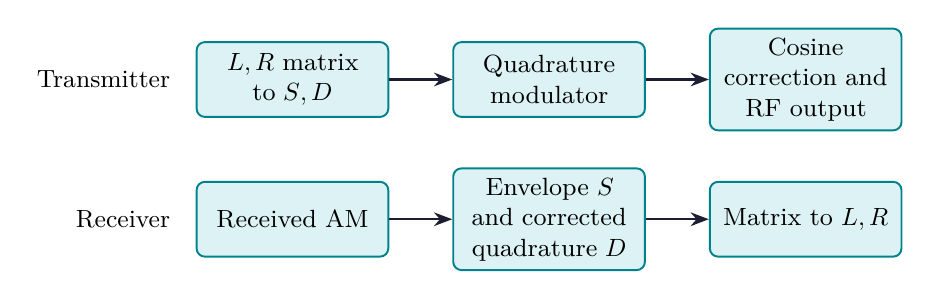
\begin{tikzpicture}[node distance=8mm,sblock/.style={block,text width=2.2cm}]
  \node[sblock] (m) {$L,R$ matrix to $S,D$};
  \node[sblock,right=of m] (q) {Quadrature modulator};
  \node[sblock,right=of q] (tx) {Cosine correction and RF output};
  \draw[arrow] (m)--(q); \draw[arrow] (q)--(tx);
  \node[sblock,below=8mm of m] (rf) {Received AM};
  \node[sblock,right=of rf] (de) {Envelope $S$ and corrected quadrature $D$};
  \node[sblock,right=of de] (lr) {Matrix to $L,R$};
  \draw[arrow] (rf)--(de); \draw[arrow] (de)--(lr);
  \node[anchor=east] at ([xshift=-2mm]m.west) {\small Transmitter};
  \node[anchor=east] at ([xshift=-2mm]rf.west) {\small Receiver};
\end{tikzpicture}\par
\end{tcolorbox}
\par\smallskip
{\small See these stereo and multiplex references.

\href{https://patents.google.com/patent/US4170716A/en}{Motorola compatible AM stereo receiver}
and \href{https://www.itu.int/rec/R-REC-BS.450/en}{ITU-R BS.450}.\par}

\section{Random Signals and Noise in Communication}
\subsection{Noise Sources and Random Processes}
A random process $X(t)$ is a family of random variables indexed by time. Each realization is a waveform. A wide-sense stationary process has constant mean and autocorrelation depending only on lag, $R_X(\tau)=E[X(t)X(t+\tau)]$ for real $X$. Its power spectral density (PSD) is the Fourier transform of $R_X(\tau)$. An LTI filter changes an input PSD $S_X$ to $|H(f)|^2 S_X(f)$.

\par\vspace{6pt}
\begingroup
\setlength{\extrarowheight}{3pt}
\noindent\begin{tabularx}{\linewidth}{|B{3.3cm}|Y|Y|}
\hline
\multicolumn{1}{|c|}{\textbf{Class}} & \multicolumn{1}{c|}{\textbf{Origins}} & \multicolumn{1}{c|}{\textbf{Engineering response}}\\
\hline
External & Atmospheric lightning, solar and galactic radiation, industrial and switching interference. & Antenna placement, shielding, grounding and RF selectivity.\\
\hline
Internal & Thermal agitation, shot noise from discrete charge flow and low-frequency flicker noise. & Low-noise front end, suitable bias and limited noise bandwidth.\\
\hline
\end{tabularx}\par
\endgroup

\subsection{White Noise, Thermal Noise and Noise Temperature}
\begin{tcolorbox}[formulabox, title={Noise Power and SNR}]
White noise has constant PSD across the band of interest. With a two-sided PSD $N_0/2$, ideal white noise passed by an LPF of cutoff $W$ has power $N_0 W$. Ideal whiteness over infinite bandwidth is a model. AWGN means additive, white and Gaussian noise. Gaussian describes the amplitude distribution, whereas whiteness describes the spectrum.

For a resistor at temperature $T$, the classical one-sided open-circuit voltage PSD is $4kTR$ in $\mathrm{V^2/Hz}$. A matched load sees half the open-circuit voltage. Across bandwidth $B$,
\[
\begin{aligned}
 \overline{v_{\rm load}^2}&=\frac{4kTRB}{4}=kTRB,\\
 P_N&=\frac{\overline{v_{\rm load}^2}}{R}=kTB\quad(\mathrm W),\\
 \mathrm{SNR}&=\frac{P_s}{P_N},\quad
 \mathrm{SNR}_{\rm dB}=10\log_{10}(P_s/P_N).
\end{aligned}
\]
Here $k=1.380649\times10^{-23}\,\mathrm{J/K}$. Use equivalent noise bandwidth for a nonrectangular filter.
\end{tcolorbox}

Equivalent input noise temperature $T_e$ expresses receiver-added noise as an input source $kT_eB$. For source noise temperature $T_A$, input-referred system noise is $k(T_A+T_e)B$. Noise factor $F$ is input SNR divided by output SNR at the standard reference temperature $T_0=290\,\mathrm K$:
\[
 F=\frac{\mathrm{SNR}_{\rm in}}{\mathrm{SNR}_{\rm out}}=1+\frac{T_e}{T_0},\qquad \mathrm{NF}_{\rm dB}=10\log_{10}F.
\]
For a cascade of $n$ amplifier stages with available gains $G_1, G_2, \dots$ and noise figures $F_1, F_2, \dots$, \textbf{Friis' Formulas} express overall noise performance:
\[
\begin{aligned}
 F_{\rm sys} &= F_1 + \frac{F_2 - 1}{G_1} + \frac{F_3 - 1}{G_1 G_2} + \dots + \frac{F_n - 1}{G_1 G_2 \cdots G_{n-1}},\\
 T_{e,\rm sys} &= T_{e1} + \frac{T_{e2}}{G_1} + \frac{T_{e3}}{G_1 G_2} + \dots + \frac{T_{en}}{G_1 G_2 \cdots G_{n-1}}.
\end{aligned}
\]
\textit{Key Architectural Consequence}: The first stage noise figure $F_1$ and equivalent temperature $T_{e1}$ directly enter the sum unattenuated, while noise from subsequent stages is divided by the preceding linear gains ($G_1, G_1G_2, \dots$). Therefore, a high-gain, low-noise pre-amplifier (LNA) placed as the first receiver stage renders all downstream stage noise contributions virtually negligible.

\begin{tcolorbox}[examplebox, title={Noise Temperature and Input-Referred SNR}]
A receiver has $F=2$, an antenna has $T_A=150\,\mathrm K$, and $B=10\,\mathrm{kHz}$. Received signal power is $10^{-13}\,\mathrm W$.
\[
\begin{aligned}
 T_e&=(2-1)(290)=290\,\mathrm K,\\
 T_{\rm sys}&=150+290=440\,\mathrm K,\\
 P_N&=(1.380649\times10^{-23})(440)(10^4)\,\mathrm W\\
    &\approx6.07\times10^{-17}\,\mathrm W,\\
 \mathrm{SNR}_{\rm dB}&=10\log_{10}\!\left(\frac{10^{-13}}{6.07\times10^{-17}}\right)
             \approx32.2\,\mathrm{dB}.
\end{aligned}
\]
\end{tcolorbox}

\begin{tcolorbox}[examplebox, title={Calculate a Two-Stage Receiver Noise Temperature}]
The first amplifier has gain $G_1=10$ and input-referred noise temperature $T_{e1}=70\,\mathrm K$. The converter that follows has $T_{e2}=400\,\mathrm K$.
\[
\begin{aligned}
 T_e &= T_{e1}+\frac{T_{e2}}{G_1}
      =70+\frac{400}{10}=110\,\mathrm K,\\
 F&=1+\frac{T_e}{290}=1.379,\qquad
 NF=10\log_{10}F\approx1.40\,\mathrm{dB}.
\end{aligned}
\]
With an antenna at $120\,\mathrm K$, the total input-referred system temperature is $230\,\mathrm K$. For a $200\,\mathrm{kHz}$ noise bandwidth the available noise is
\[
 P_N=k(230)(200\,000)\approx6.35\times10^{-16}\,\mathrm W.
\]
The later converter contributes only $40\,\mathrm K$ referred to the input because the preceding amplifier has gain ten. In cascade formulas use linear gain and noise factor, then convert to decibels if required.
\end{tcolorbox}

\section{Noise Performance of Analog Modulation}
\subsection{Reference SNR and Detection Assumptions}
Let $W$ be the baseband bandwidth and $N_0/2$ the two-sided RF noise PSD. Express powers at a normalized $1\,\Omega$ load. Let $P_R$ be total received RF signal power, including any transmitted carrier, and $P_U$ its information-bearing RF power. Use the same baseband reference for every scheme:
\[
 \gamma_{\rm ref}=\frac{P_R}{N_0W},\qquad
 \mathcal F=\frac{\mathrm{SNR}_{\rm out}}{\gamma_{\rm ref}}.
\]
This figure of merit $\mathcal F$ uses a common reference rather than actual RF-filter input SNR. A rectangular RF filter of positive-frequency bandwidth $B_{\rm RF}$ passes noise power $N_0B_{\rm RF}$, giving actual RF input SNR $P_R/(N_0B_{\rm RF})$. If a question uses that denominator, multiply $\mathcal F$ by $B_{\rm RF}/W$.

\subsection{DSB-TC, DSB-SC, SSB-TC and SSB-SC}
Ideal coherent detection uses $2\cos(2\pi f_ct)$ and a baseband LPF. For DSB, the shifted positive and negative RF noise bands both contribute across $|f|\le W$. Thus $S_{n,\rm out}=N_0$, giving $2N_0W$. The useful waveform $u(t)\cos\omega_ct$ has $P_U=E[u^2]/2$. Its baseband useful power is $E[u^2]=2P_U$, so
\[
 \mathrm{SNR}_{\rm out,DSB}=\frac{2P_U}{2N_0W}=\frac{P_U}{N_0W}.
\]
For DSB-TC the carrier becomes DC and is removed. At high carrier-to-noise ratio with a positive envelope, the envelope detector also yields the in-phase noise to first order. For the single tone, $P_U/P_R=\mu^2/(2+\mu^2)$. DSB-SC uses all of $P_R$ for the useful sidebands.

For SSB, $s_U(t)=u(t)\cos\omega_ct-\widehat u(t)\sin\omega_ct$. With zero-mean $u$, the Hilbert transform has the same power, so
\[
 P_U=\tfrac12[E(u^2)+E(\widehat u^2)]=E(u^2).
\]
Only one translated noise contribution remains at each nonzero baseband frequency, giving $S_{n,\rm out}=N_0/2$ and $N_0W$ in-band noise. Coherent SSB detection therefore also gives $P_U/(N_0W)$. SSB-SC has $P_R=P_U$. SSB-TC has $P_R=P_U+P_c$. The carrier becomes removable DC. A strong-carrier envelope detector can approximate coherent output to first order, with quadrature distortion as the carrier becomes less dominant.

\begin{tcolorbox}[formulabox, title={Track the RF Noise through the Product Detector}]
The oscillator $2\cos(2\pi f_ct)$ translates RF noise to baseband through two unit-amplitude frequency shifts. For filtered, wide-sense stationary noise with RF PSD $S_{n,\rm RF}$, the time-averaged baseband PSD is
\[
 S_{n,\rm out}(f)=S_{n,\rm RF}(f-f_c)+S_{n,\rm RF}(f+f_c),
 \qquad |f|\le W .
\]
The two separated RF contributions have uncorrelated spectral increments. A DSB RF filter passes both terms at each in-band $f$, yielding $N_0$. An SSB RF filter passes one, yielding $N_0/2$. The carrier line in a transmitted-carrier scheme shifts to DC and is removed when calculating useful audio power.
\end{tcolorbox}

\begin{tcolorbox}[examplebox, title={Keep Reference SNR and RF Input SNR Separate}]
For DSB-TC, let $P_R=2\,\mathrm{mW}$, $W=4\,\mathrm{kHz}$, $N_0=5\times10^{-10}\,\mathrm{W/Hz}$ and tone index $\mu=0.5$. The RF filter has $B_{\rm RF}=2W$.
\[
\begin{aligned}
 \gamma_{\rm ref} &=\frac{2\times10^{-3}}{(5\times10^{-10})(4000)}=1000,\\
 \gamma_{\rm RF,in}&=\frac{2\times10^{-3}}{(5\times10^{-10})(8000)}=500,\\
 \eta &= \frac{\mu^2}{2+\mu^2}=\frac19,\\
 \gamma_{\rm out}&=\eta\gamma_{\rm ref}=\frac{1000}{9}\approx111.1 .
\end{aligned}
\]
The figure of merit under the common-reference convention is $1/9$. Under the actual RF input convention it is $111.1/500\approx2/9$. The receiver and its output SNR are the same in both calculations.
\end{tcolorbox}

\subsection{FM Discriminator Noise Above Threshold}
A limiter removes amplitude variations. Let the received FM amplitude be $A$, so that $P_R=A^2/2$. For high predetection carrier-to-noise ratio, received quadrature noise $n_Q(t)$ gives a small phase error $n_Q/A$. Ideal broad predetection filtering gives quadrature noise PSD approximately $N_0$ over the output band. A unity-frequency-gain discriminator followed by scaling by $1/k_f$ gives the output $m(t)$ plus
\[
\begin{aligned}
 n_o(t)&\approx \frac{1}{2\pi A k_f}\frac{d n_Q(t)}{dt},\\
 S_{n_o}(f)&\approx \frac{N_0 f^2}{A^2 k_f^2},\qquad |f|\le W,\\
 P_{n_o}&=\int_{-W}^{W}S_{n_o}(f)\,df
          =\frac{2N_0 W^3}{3A^2k_f^2},\\
 \mathrm{SNR}_{\rm out,FM}
      &\approx\frac{3P_Rk_f^2P_m}{N_0W^3},
      \qquad P_m=E[m^2(t)].
\end{aligned}
\]
For a full-band tone with $f_m=W$, $P_m=A_m^2/2$ and $\Delta f=k_f A_m$. Hence $\mathcal F_{\rm FM}\approx\tfrac32(\Delta f/W)^2$. The noise voltage density grows with frequency, and noise PSD grows as $f^2$. Pre-emphasis boosts high audio frequencies before transmission and complementary de-emphasis reduces their noise after detection. Below threshold, large phase errors produce clicks and the small-noise formula no longer applies.

\begin{tcolorbox}[tikzbox, unbreakable, title={FM Discriminator Output Noise PSD}]
\centering
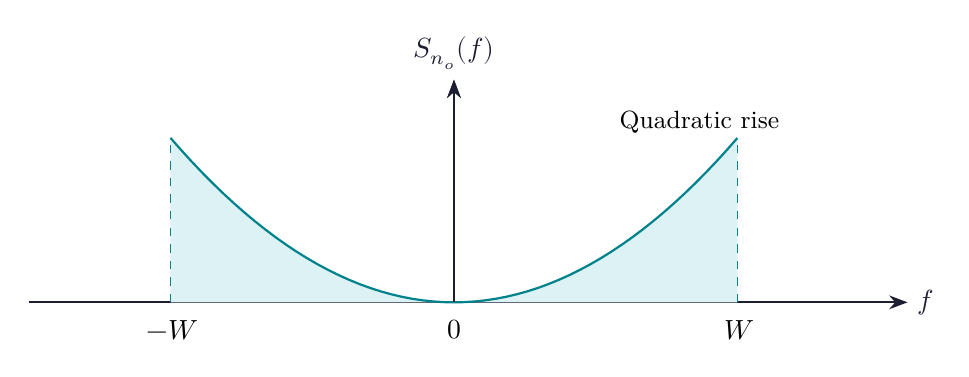
\begin{tikzpicture}[x=1.8cm,y=1.45cm]
  \draw[arrow] (-3,0)--(3.2,0) node[right] {$f$};
  \draw[arrow] (0,0)--(0,1.95) node[above] {$S_{n_o}(f)$};
  \fill[hdrteal,domain=-2:2,samples=55] (-2,0)--plot (\x,{0.36*\x*\x})--(2,0)--cycle;
  \draw[myteal,thick,domain=-2:2,samples=55] plot (\x,{0.36*\x*\x});
  \draw[dashed,myteal] (-2,0)--(-2,1.44) (2,0)--(2,1.44);
  \draw[arrow] (0,0)--(0,1.95);
  \node[below=3pt] at (-2,0) {$-W$};
  \node[below=3pt] at (0,0) {$0$};
  \node[below=3pt] at (2,0) {$W$};
  \node[right] at (1.1,1.58) {\small Quadratic rise};
\end{tikzpicture}\par
\end{tcolorbox}

\begin{tcolorbox}[examplebox, title={Compare Five Schemes at Equal Total Received Power}]
Let $\gamma_{\rm ref}=100$ ($20\,\mathrm{dB}$). Use conventional AM with $\mu=0.8$, SSB-TC with $P_c=3P_U$, and full-band tone FM with $\Delta f/W=4$ above threshold. Under the respective detection assumptions:
\[
\begin{aligned}
 \gamma_{\rm DSB-TC}&=100\frac{0.8^2}{2+0.8^2}
          \approx24.24\quad(13.85\,\mathrm{dB}),\\
 \gamma_{\rm DSB-SC}&=100\quad(20\,\mathrm{dB}),\\
 \gamma_{\rm SSB-TC}&=100\frac{1}{1+3}
          =25\quad(13.98\,\mathrm{dB}),\\
 \gamma_{\rm SSB-SC}&=100\quad(20\,\mathrm{dB}),\\
 \gamma_{\rm FM}&\approx100\left(\frac32\right)4^2
          =2400\quad(33.80\,\mathrm{dB}).
\end{aligned}
\]
The FM improvement uses a larger RF bandwidth. Carrier suppression avoids using part of the total power in a non-message component.
\end{tcolorbox}
\par\smallskip
{\small Further reading on figure of merit and detector noise.

\href{https://archive.nptel.ac.in/content/storage2/courses/117106090/Pdfs/1_10.pdf}{IIT Madras Principles of Communication noise analysis}.\par}

\section{Probability and Signal Distributions}
\subsection{Joint Probability, Conditioning and Independence}
For $P(B)>0$, the joint probability of $A$ and $B$ and its conditional form obey
\[
 P(A\cap B)=P(A\mid B)P(B),\qquad
 P(A\mid B)=\frac{P(A\cap B)}{P(B)}.
\]
Independence means $P(A\cap B)=P(A)P(B)$. For two random variables it means the joint CDF factors. Where joint densities exist, the joint density equals the product of marginals almost everywhere. Summing a joint PMF or integrating a joint PDF over one variable gives the other marginal.

\begin{tcolorbox}[examplebox, title={Infer a Transmitted Bit from the Detected Bit}]
Let $P(T=1)=0.3$, $P(R=1\mid T=1)=0.9$, and $P(R=1\mid T=0)=0.1$.
\[
\begin{aligned}
 P(T=1,R=1)&=0.9(0.3)=0.27,\\
 P(R=1)&=0.9(0.3)+0.1(0.7)=0.34,\\
 P(T=1\mid R=1)&=\frac{0.27}{0.34}\approx0.794.
\end{aligned}
\]
Since $P(T=1\mid R=1)\ne P(T=1)$, the detected and transmitted bits are statistically dependent.
\end{tcolorbox}

\subsection{Discrete and Continuous Random Variables}
A discrete random variable has a probability mass function (PMF) $p_X(x)=P(X=x)$. For a continuous variable with density $f_X$, probabilities are integrals of nonnegative density, with total integral one. A density has units inverse to the variable units. The cumulative distribution function (CDF) is always $F_X(x)=P(X\le x)$:
\[
 \begin{aligned}
 F_X(x)&=\sum_{x_i\le x}p_X(x_i) && \text{(discrete)},\\
 F_X(x)&=\int_{-\infty}^{x}f_X(u)\,du && \text{(continuous)},\\
 P(a<X\le b)&=F_X(b)-F_X(a).
 \end{aligned}
\]
For a differentiable continuous CDF, $f_X=F_X'$. A discrete CDF jumps at each point of positive mass. A continuous variable with a PDF has $P(X=x)=0$ at a single point.

\subsection{Gaussian, Rayleigh and Rician Densities}
\begin{tcolorbox}[formulabox, title={Three Communication Distributions}]
\textbf{Gaussian.} For mean $\mu$ and variance $\sigma^2$, the PDF is
\[
 f_X(x)=\frac{1}{\sigma\sqrt{2\pi}}\exp\!\left[-\frac{(x-\mu)^2}{2\sigma^2}\right],
 \qquad -\infty<x<\infty.
\]
The CDF is $F_X(x)=\Phi((x-\mu)/\sigma)$, with $\Phi$ the standard normal CDF. Gaussian noise is used for receiver thermal noise.

\textbf{Rayleigh.} With independent zero-mean Gaussian quadratures of variance $\sigma^2$, their envelope $R=\sqrt{I^2+Q^2}$ is Rayleigh. Transforming to polar coordinates multiplies the joint density by the Jacobian $r$. Integrating the angle over $2\pi$ gives
\[
 f_R(r)=\frac{r}{\sigma^2}e^{-r^2/(2\sigma^2)},\qquad
 F_R(r)=1-e^{-r^2/(2\sigma^2)},\qquad r\ge0.
\]
Both are zero for $r<0$. This envelope model is used for diffuse multipath without a dominant component.

\textbf{Rician.} With a deterministic phasor of magnitude $a$ and diffuse Gaussian quadratures of variance $\sigma^2$ each,
\[
 f_R(r)=\frac{r}{\sigma^2}
        e^{-(r^2+a^2)/(2\sigma^2)} I_0\!\left(\frac{ra}{\sigma^2}\right),
        \qquad r\ge0.
\]
The PDF is zero for negative $r$. Here $I_0$ is the modified Bessel function of order zero, arising from angular integration of the shifted Gaussian density. The CDF is $\int_0^r f_R(u)\,du$ for $r\ge0$. The ratio of deterministic to diffuse power is $K=a^2/(2\sigma^2)$. At $a=0$, $I_0(0)=1$ and the density becomes Rayleigh.
\end{tcolorbox}

\subsection{Derive the Envelope Distributions from Gaussian Quadratures}
For independent quadrature voltages $I,Q\sim\mathcal N(0,\sigma^2)$, write $i=r\cos\theta$ and $q=r\sin\theta$. The area element changes from $di\,dq$ to $r\,dr\,d\theta$. Therefore the joint density of radius and angle and its marginal are
\[
\begin{aligned}
 f_{R,\Theta}(r,\theta)
   &=\frac{r}{2\pi\sigma^2}\exp[-r^2/(2\sigma^2)],\\
 f_R(r)&=\int_0^{2\pi} f_{R,\Theta}(r,\theta)\,d\theta
        =\frac{r}{\sigma^2}e^{-r^2/(2\sigma^2)},\\
 F_R(r)&=\int_0^r\frac{u}{\sigma^2}e^{-u^2/(2\sigma^2)}\,du
        =\left[-e^{-u^2/(2\sigma^2)}\right]_0^r .
\end{aligned}
\]
Now choose the in-phase axis along a deterministic phasor so $I\sim\mathcal N(a,\sigma^2)$ and $Q\sim\mathcal N(0,\sigma^2)$ remain independent. The shifted quadratic becomes
\[
 (i-a)^2+q^2=r^2+a^2-2ra\cos\theta.
\]
After the same Jacobian and angular integration,
\[
\begin{aligned}
 f_R(r)&=\frac r{\sigma^2}e^{-(r^2+a^2)/(2\sigma^2)}
          \left[\frac{1}{2\pi}\int_0^{2\pi}
                 e^{(ra/\sigma^2)\cos\theta}\,d\theta\right],\\
       &=\frac r{\sigma^2}e^{-(r^2+a^2)/(2\sigma^2)}
                       I_0(ra/\sigma^2),\qquad r\ge0.
\end{aligned}
\]
This is the Rician density. Setting $a=0$ makes the bracket one and gives the Rayleigh density. The Gaussian model describes the signed quadrature voltages. Their nonnegative magnitude follows the envelope model.

\begin{tcolorbox}[tikzbox, unbreakable, title={Gaussian, Rayleigh and Rician Density Shapes}]
\centering
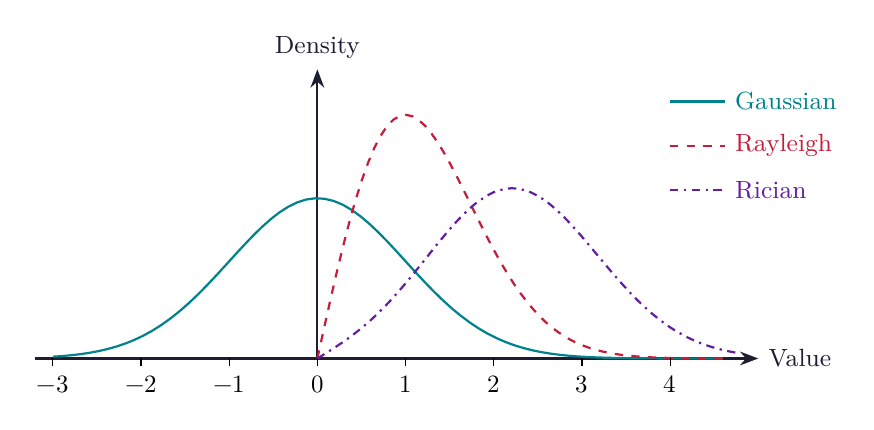
\begin{tikzpicture}[x=1.12cm,y=5.1cm,every node/.style={font=\small}]
  \draw[arrow] (-3.2,0)--(5.0,0) node[right] {Value};
  \draw[arrow] (0,0)--(0,0.72) node[above] {Density};
  \draw[myteal,thick,domain=-3:4.6,samples=75] plot (\x,{0.398942*exp(-\x*\x/2)});
  \draw[myred,thick,dashed,domain=0:4.6,samples=65] plot (\x,{\x*exp(-\x*\x/2)});
  \draw[mypurple,thick,dashdotted] plot[smooth] coordinates {
    (0.0,0.0000) (0.2,0.0276) (0.4,0.0583) (0.6,0.0945) (0.8,0.1376) (1.0,0.1871) (1.2,0.2410) (1.4,0.2956) (1.6,0.3460)
    (1.8,0.3870) (2.0,0.4140) (2.2,0.4239) (2.4,0.4156) (2.6,0.3904) (2.8,0.3514) (3.0,0.3032) (3.2,0.2509)
    (3.4,0.1992) (3.6,0.1516) (3.8,0.1108) (4.0,0.0776) (4.2,0.0522) (4.4,0.0337) (4.6,0.0209) (4.8,0.0124)
  };
  \foreach \x in {-3,-2,-1,0,1,2,3,4}{
    \draw (\x,0)--(\x,-0.018) node[below] {$\x$};
  }
  \draw[myteal,thick] (4,0.64)--(4.62,0.64) node[right] {Gaussian};
  \draw[myred,thick,dashed] (4,0.53)--(4.62,0.53) node[right] {Rayleigh};
  \draw[mypurple,thick,dashdotted] (4,0.42)--(4.62,0.42) node[right] {Rician};
\end{tikzpicture}\par
\small Here $\sigma=1$ in all three models, $\mu=0$ for the Gaussian, and $a=2$ for the Rician. The Gaussian can take negative values. The envelope distributions start at zero.
\end{tcolorbox}

\begin{tcolorbox}[examplebox, title={Rayleigh Envelope Outage}]
For Rayleigh quadrature scale $\sigma=1\,\mathrm V$ and a receiver threshold $r_0=0.5\,\mathrm V$,
\[
 P(R<r_0)=F_R(r_0)=1-e^{-(0.5)^2/2}\approx0.1175.
\]
Roughly $11.75\%$ of envelope samples fall below the threshold under this model.
\end{tcolorbox}

\begin{tcolorbox}[masonbox, title={Exam Checks}]
Use actual RF noise bandwidth for RF-filter noise power and the stated reference bandwidth for figure of merit. Convert power ratios with $10\log_{10}$. State the limiting assumptions for envelope or FM noise analysis. For amplitude statistics, distinguish the Gaussian quadratures from their nonnegative envelope.
\end{tcolorbox}


\newpage
\begin{center}
  {\large\bfseries\color{myred} Quick Revision --- Module 4}\\[3pt]
  {\small\color{mydark} Multiplexing, Stereo, Random Signals and Noise $|$ EC401}
\end{center}
\noindent{\color{myred}\rule{\linewidth}{1.2pt}}
\par\vspace{4pt}

\begin{tcolorbox}[formulabox, title={Key Formulas at a Glance}]
\renewcommand{\arraystretch}{1.35}
\noindent\begin{tabularx}{\linewidth}{B{4.4cm} Y}
FDM and TDM & $B_{\rm span}=NB_{\rm ch}+(N-1)g$ \newline $R_{\rm slot}=(N+n_{\rm ov})f_s$ \\[4pt]
Stereo matrix & $S=L+R,\ D=L-R$ \newline $L=(S+D)/2,\ R=(S-D)/2$ \\[4pt]
Thermal noise & $P_N=kTB$ \quad $T_e=(F-1)T_0$ \\[4pt]
AM and SSB output SNR & $P_U/(N_0W)$ under the stated detection assumptions \\[4pt]
FM above threshold & $\mathrm{SNR}_{\rm out}\approx3P_R k_f^2P_m/(N_0 W^3)$ \\[4pt]
Conditional probability & $P(A\mid B)=P(A\cap B)/P(B)$ \\[4pt]
Rayleigh CDF & $F_R(r)=1-\exp[-r^2/(2\sigma^2)]$ for $r\ge0$ \\[4pt]
\end{tabularx}\par
\end{tcolorbox}

\begin{tcolorbox}[defbox, title={One-Line Definitions}]
\begin{itemize}[leftmargin=*, itemsep=3pt, topsep=0pt]
  \item \textbf{Guard band.} Frequency gap between neighbouring FDM allocations.
  \item \textbf{Frame.} Recurring group of slots with one sample per channel in synchronous PAM-TDM.
  \item \textbf{Noise temperature.} Input equivalent temperature representing added noise.
  \item \textbf{Rayleigh envelope.} Magnitude of two independent zero-mean Gaussian quadratures of equal variance.
\end{itemize}
\end{tcolorbox}

\begin{tcolorbox}[exambox, title={Frequently Asked / Viva Questions}]
\begin{enumerate}[topsep=0pt, label=\textbf{Q\arabic*.}, itemsep=5pt]
  \item \Q{Why does FDM need guard bands?}
    Practical filters need transition width to limit leakage between adjacent bands.
  \item \Q{What does TDM require at the receiver?}
    A timing reference for slot decisions and frame synchronization for channel identification.
  \item \Q{How does mono FM remain compatible with stereo FM?}
    The mono receiver uses the low-pass $L+R$ signal. A stereo receiver additionally detects $L-R$.
  \item \Q{How is a mono AM signal retained in C-QUAM?}
    Cosine correction makes the RF envelope proportional to the biased sum channel $1+k_s(L+R)$.
  \item \Q{Are white and Gaussian equivalent descriptions?}
    White specifies the spectrum. Gaussian specifies an amplitude distribution.
  \item \Q{What is available thermal noise power?}
    A matched load gets $kTB$ from a source at temperature $T$ over noise bandwidth $B$.
  \item \Q{Why does adding a carrier lower AM figure of merit?}
    It increases $P_R$ but contributes no message power $P_U$. The ratio under the common reference is $P_U/P_R$.
  \item \Q{Why does FM noise increase at high audio frequencies?}
    The discriminator differentiates phase noise, multiplying its PSD by a factor proportional to $f^2$.
  \item \Q{When are two events independent?}
    When $P(A\cap B)=P(A)P(B)$.
  \item \Q{How does a Rician model reduce to Rayleigh?}
    Set deterministic amplitude $a=0$, so $K=0$ and $I_0(0)=1$.
\end{enumerate}
\end{tcolorbox}

\begin{tcolorbox}[tikzbox, unbreakable, title={Summary Comparison}]
\begingroup
\setlength{\tabcolsep}{5pt}
\setlength{\extrarowheight}{3pt}
\renewcommand{\arraystretch}{1.45}
\noindent\begin{tabularx}{\linewidth}{|B{3.35cm}|Y|Y|}
\hline
\multicolumn{1}{|c|}{\textbf{Scheme}} & \multicolumn{1}{c|}{\textbf{Output SNR}} & \multicolumn{1}{c|}{\textbf{Common-reference figure of merit}} \\
\hline
DSB-TC & $P_U/(N_0W)$ & $\mu^2/(2+\mu^2)$ for a tone \\
\hline
DSB-SC & $P_R/(N_0W)$ & $1$ \\
\hline
SSB-TC & $P_U/(N_0W)$ & $P_U/(P_U+P_c)$ \\
\hline
SSB-SC & $P_R/(N_0W)$ & $1$ \\
\hline
FM & $3P_Rk_f^2P_m/(N_0W^3)$ & $\tfrac32(\Delta f/W)^2$ for a full-band tone above threshold \\
\hline
\end{tabularx}\par
\endgroup
\end{tcolorbox}


\end{document}
